\chapter{ANALYSIS STRATEGY} \label{strategy}

The first \VHbb\ analysis conducted by the CMS collaboration in 2012\cite{HIG13012} demonstrated that an observation of the \Hbb\ decay was feasible by combining searches for the \ZnnHbb, \WenHbb, \WmnHbb, \ZeeHbb, and \ZmmHbb\ decay channels. The overall strategy that it pioneered has remained largely intact, even through the transition to LHC Run 2. The search for \VHbb\ using the 2016 dataset would establish evidence for the \Hbb\ decay in 2017\cite{CMSVHbbEvidence} with only incremental improvements. The search for \VHbb\ using the 2017 dataset would build on the physics insights and experiences obtained the year prior while bringing to bear additional event reconstruction techniques and deep learning to finally observe the \Hbb\ decay in 2018.\cite{HIG18016} This chapter describes the analysis strategy used by CMS to achieve its state of the art result, with a focus on the \ZnnHbb\ decay channel in particular.\footnote{This chapter includes content adapted from Ref. \cite{CMSVHbbEvidence} and \cite{HIG18016}, as the author's work directly contributed to those publications.}

\section{Data and Simulation}

\subsection{Data}

The datasets used for this analysis were collected by the CMS detector throughout 2017 and produced by proton-proton collisions with a center-of-mass energy $\sqrt{s} = 13\ \TeV$ and a bunch spacing of 25 ns. The \ZnnH\ channel uses the MET dataset, the \WenH\ channel uses the SingleElectron dataset, the \WmnH\ channel uses the SingleMuon dataset, the \ZeeH\ channel uses the DoubleEG dataset, and the \ZmmH\ channel uses the DoubleMuon dataset. All of these primary datasets have an approximate total luminosity of 41.3 \invfb\ when only considering \textit{golden} events, which were certified by data quality monitoring teams to have been collected during periods of normal function for all detector subsystems. The JSON certification file \texttt{Cert\_294927-306462\_13TeV\_EOY2017ReReco\_Collisions17\_JSON\_v1.txt} was used to filter for golden events.

\subsection{Simulation}

Simulated samples for each of the relevant signal and background processes are used to design and validate the analysis strategy in an unbiased manner. These samples are produced using different Monte-Carlo (MC) generators and processed by the \textsc{\small GEANT4}\cite{GEANT4A,GEANT4B,GEANT4C} software which realistically models the detector's response to the passage of particles through its materials. The reconstruction of these MC events was performed using CMS SoftWare (CMSSW) version 94X releases set to match the 2017 data taking conditions.

The signal samples, generated using the \textsc{\small POWHEG} v2\cite{POWHEGA,POWHEGB,POWHEGC} event generator, are listed in Table \ref{tbl:MCsignal}. The quark-induced signal processes are generated to next-to-leading order (NLO) accuracy in QCD using the MiNLO procedure \cite{MINLOA,MINLOB}, while the gluon-induced contributions to the $ZH$ signal processes are generated only to leading order (LO) accuracy in QCD. Their production cross sections and branching fractions are taken to be the state of the art values calculated for a Higgs boson mass of $\massH = 125\ \GeV$ from Ref. \cite{CERNYR4}, and specifically those listed in sections \ref{productionmodes} and \ref{decaymodes}. These production cross sections are further rescaled to next-to-next-to-leading order (NNLO) accuracy in QCD and NLO electroweak accuracy as a function of the transverse momentum of the vector boson \pTV, according to the combined calculations of the \textsc{\small VHNNLO}\cite{VHNNLOA,VHNNLOB,VHNNLOC,VHNNLOD}, \textsc{\small VH@NNLO}\cite{VHATNNLOA,VHATNNLOB}, and \textsc{\small HAWK} v2.0\cite{HAWK} event generators as described in Ref. \cite{CERNYR4}. The event weights used to rescale the samples are specific to each signal process and an example of the weights applied to the $\bosWp(\ell\nu)\Htobb$ channel are shown in Figure \ref{fig:VHNNLOweight}.

\begin{table}[htbp]
  \caption[Signal Samples for \VHbb\ 2017]{The Monte-Carlo samples and their cross sections for the signal processes considered by the 2017 \VHbb\ analysis.}
  \label{tbl:MCsignal}
  \small
  \begin{tabularx}{6.5in}{lX}
    \hline
    Sample                                                        & $\sigma (\pb)$                                   \\
    \hline
    \texttt{WminusH\_HToBB\_WToLNu\_M125\_13TeV\_powheg\_pythia8} & $0.5824 \times 0.533 \times 0.108535$            \\
    \texttt{WplusH\_HToBB\_WToLNu\_M125\_13TeV\_powheg\_pythia8}  & $0.5824 \times 0.840 \times 0.108535$            \\
    \texttt{ZH\_HToBB\_ZToLL\_M125\_13TeV\_powheg\_pythia8}       & $0.5824 \times (0.8839 - 0.1227) \times 0.10974$ \\
    \texttt{ZH\_HToBB\_ZToNuNu\_M125\_13TeV\_powheg\_pythia8}     & $0.5824 \times (0.8839 - 0.1227) \times 0.20103$ \\
    \texttt{ggZH\_HToBB\_ZToLL\_M125\_13TeV\_powheg\_pythia8}     & $0.5824 \times 0.1227 \times 0.10974$            \\
    \texttt{ggZH\_HToBB\_ZToNuNu\_M125\_13TeV\_powheg\_pythia8}   & $0.5824 \times 0.1227 \times 0.20103$            \\
    \hline
  \end{tabularx}
\end{table}

\begin{figure}[htbp]
  \centering
    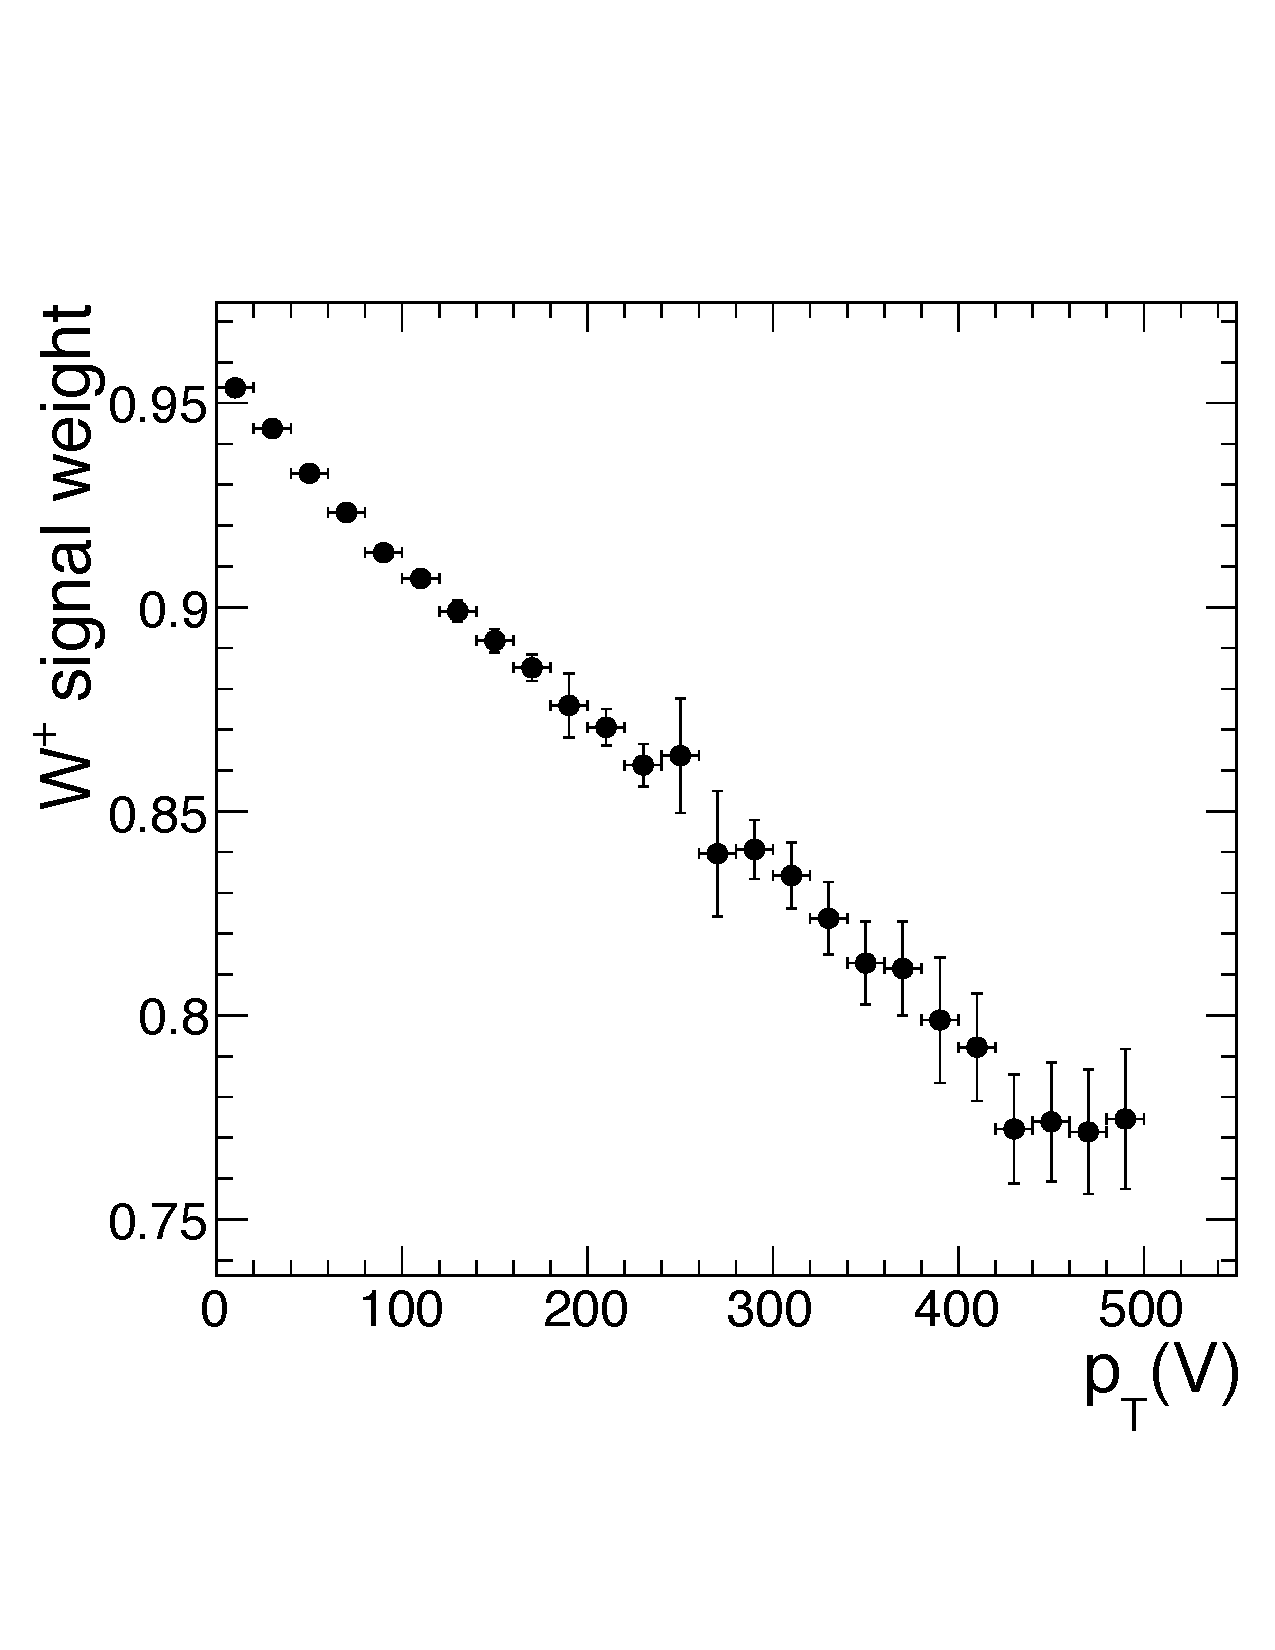
\includegraphics[width=3in]{images/ewk_wplush_correction}
    \caption[2017 Signal MC Rescaling Weights for $\bosWp(\ell\nu)\Htobb$]{The event weights used to rescale the production cross section of the $\bosWp(\ell\nu)\Htobb$ signal Monte-Carlo sample to NNLO QCD and NLO electroweak accuracy.}
    \label{fig:VHNNLOweight}
\end{figure}

The diboson samples listed in Table \ref{tbl:MCdiboson} are generated using the \textsc{\small MadGraph5\_amc@NLO} v2.4.2\cite{AMCNLO} event generator at NLO accuracy with the FxFx\cite{FXFX} merging scheme and up to two additional partons. The exception is the inclusive \bosZ\bosZ\ sample which is only simulated to LO accuracy and generated using \textsc{\small PYTHIA} v8.230\cite{PYTHIA8} event generator. Although the cross section of the \texttt{ZZTo2L2Q} sample has been obtained from an NLO calculation, the other cross sections are taken to be the product of their measured inclusive cross sections\cite{WWxsec,WZxsec,ZZxsec} and the appropriate branching ratio as computed by the Particle Data Group (PDG) in Ref. \cite{PDG2018}.

\begin{table}[htbp]
  \caption[Diboson Samples for \VHbb\ 2017]{The Monte-Carlo samples and their cross sections for the diboson processes considered by the 2017 \VHbb\ analysis.}
  \label{tbl:MCdiboson}
  \begin{tabularx}{6.5in}{lX}
    \hline
    Sample                                                      & $\sigma (\pb)$ \\
    \hline
    \texttt{WWTo1L1Nu2Q\_13TeV\_amcatnloFXFX\_madspin\_pythia8} & 50.86          \\
    \texttt{WZTo1L1Nu2Q\_13TeV\_amcatnloFXFX\_madspin\_pythia8} & 10.88          \\
    \texttt{ZZ\_TuneCP5\_13TeV-pythia8}                         & 14.60          \\
    \texttt{ZZTo2L2Q\_13TeV\_amcatnloFXFX\_madspin\_pythia8}    & 3.69           \\
    \hline
  \end{tabularx}
\end{table}

The \bosV+jets samples are also produced using the \textsc{\small MadGraph5\_amc@NLO} v2.4.2 event generator but at LO accuracy with the MLM matching scheme\cite{MLM}. Besides their inclusive and HT-binned configurations, \qrkb-quark enriched versions with up to four additional partons are also generated to increase the statistical power of these samples in the phase space most relevant for signal events because the \bosV+jets processes are the primary irreducible backgrounds. The samples for \bosW+jets with $\bosW \rightarrow \ell\nu$ are listed in Table \ref{tbl:MCWtoLNu}, while the samples for \bosZ+jets with $\bosZ \rightarrow \ell\bar{\ell}$ are listed in Table \ref{tbl:MCZtoLL} and with $\bosZ \rightarrow \nu\bar{\nu}$ are listed in Table \ref{tbl:MCZtoNuNu}. The cross sections of the \bosV+jets samples are multiplied by \textit{k}-factors of 1.21 and 1.23 for the \bosW+jets and \bosZ+jets samples, respectively, which rescale them to their NNLO cross sections as calculated by the \textsc{\small FEWZ} 3.1\cite{FEWZA,FEWZB,FEWZC} software. The cross sections of the \qrkb-quark enriched samples are further multiplied by a stitching factor which allows them to be used in conjunction with the inclusive and HT-binned versions by appropriately scaling their cross sections.

\begin{table}[htbp]
  \caption[\bosW+jets $(\bosW \rightarrow \ell\bar{\nu})$ Samples for \VHbb\ 2017]{The Monte-Carlo samples and their cross sections for the \bosW+jets $(\bosW \rightarrow \ell\bar{\nu})$ processes considered by the 2017 \VHbb\ analysis. Stitching factors of 1.5 and 1.12 are applied to the \texttt{WBJets} and \texttt{BGenFilter} \qrkb-quark enriched samples, respectively.}
  \label{tbl:MCWtoLNu}
  \small
  \begin{tabularx}{6.5in}{lX}
    \hline
    Sample                                                                 & $\sigma (\pb)$                 \\
    \hline
    \texttt{WJetsToLNu\_TuneCP5\_13TeV-madgraphMLM-pythia8}                & $1.21 \times 52940.0$          \\
    \texttt{WJetsToLNu\_HT-100To200\_TuneCP5\_13TeV-madgraphMLM-pythia8}   & $1.21 \times 1395.0$           \\
    \texttt{WJetsToLNu\_HT-200To400\_TuneCP5\_13TeV-madgraphMLM-pythia8}   & $1.21 \times 407.9$            \\
    \texttt{WJetsToLNu\_HT-400To600\_TuneCP5\_13TeV-madgraphMLM-pythia8}   & $1.21 \times 57.48$            \\
    \texttt{WJetsToLNu\_HT-600To800\_TuneCP5\_13TeV-madgraphMLM-pythia8}   & $1.21 \times 12.87$            \\
    \texttt{WJetsToLNu\_HT-800To1200\_TuneCP5\_13TeV-madgraphMLM-pythia8}  & $1.21 \times 5.366$            \\
    \texttt{WJetsToLNu\_HT-1200To2500\_TuneCP5\_13TeV-madgraphMLM-pythia8} & $1.21 \times 1.074$            \\
    \texttt{WJetsToLNu\_HT-2500ToInf\_TuneCP5\_13TeV-madgraphMLM-pythia8}  & $1.21 \times 0.03216$          \\
    \texttt{WBJetsToLNu\_Wpt-100to200\_TuneCP5\_13TeV-madgraphMLM-pythia8} & $1.21 \times 1.5 \times 7.35$  \\
    \texttt{WBJetsToLNu\_Wpt-200toInf\_TuneCP5\_13TeV-madgraphMLM-pythia8} & $1.21 \times 1.5 \times 1.1$   \\
    \texttt{WJetsToLNu\_BGenFilter\_Wpt-100to200\_TuneCP5\_13TeV}          & $1.21 \times 1.12 \times 26.6$ \\
    \texttt{  -madgraphMLM-pythia8}                                        &                                \\
    \texttt{WJetsToLNu\_BGenFilter\_Wpt-200toInf\_TuneCP5\_13TeV}          & $1.21 \times 1.12 \times 3.9$  \\
    \texttt{  -madgraphMLM-pythia8}                                        &                                \\
    \hline
  \end{tabularx}
\end{table}

\begin{table}[htbp]
  \caption[\bosZ+jets $(\bosZ \rightarrow \ell\bar{\ell})$ Samples for \VHbb\ 2017]{The Monte-Carlo samples and their cross sections for the \bosZ+jets $(\bosZ \rightarrow \ell\bar{\ell})$ processes considered by the 2017 \VHbb\ analysis. Stitching factors of 1.085 and 1.15 are applied to the \texttt{DYBJetsToLL} and \texttt{BGenFilter} \qrkb-quark enriched samples, respectively.}
  \label{tbl:MCZtoLL}
  \small
  \begin{tabularx}{6.5in}{lX}
    \hline
    Sample                                                              & $\sigma (\pb)$                    \\
    \hline
    \texttt{DYJetsToLL\_M-4to50\_HT-100to200\_TuneCP5\_13TeV}           & $1.23 \times 204.0$               \\
    \texttt{  -madgraphMLM-pythia8}                                     &                                   \\
    \texttt{DYJetsToLL\_M-4to50\_HT-200to400\_TuneCP5\_13TeV}           & $1.23 \times 54.4$                \\
    \texttt{  -madgraphMLM-pythia8}                                     &                                   \\
    \texttt{DYJetsToLL\_M-4to50\_HT-400to600\_TuneCP5\_13TeV}           & $1.23 \times 5.70$                \\
    \texttt{  -madgraphMLM-pythia8}                                     &                                   \\
    \texttt{DYJetsToLL\_M-4to50\_HT-600toInf\_TuneCP5\_13TeV}           & $1.23 \times 1.85$                \\
    \texttt{  -madgraphMLM-pythia8}                                     &                                   \\
    \texttt{DYJetsToLL\_M-50\_TuneCP5\_13TeV}                           & $1.23 \times 5343.0$              \\
    \texttt{  -madgraphMLM-pythia8}                                     &                                   \\
    \texttt{DYJetsToLL\_M-50\_HT-100to200\_TuneCP5\_13TeV}              & $1.23 \times 161.1$               \\
    \texttt{  -madgraphMLM-pythia8}                                     &                                   \\
    \texttt{DYJetsToLL\_M-50\_HT-200to400\_TuneCP5\_13TeV}              & $1.23 \times 48.66$               \\
    \texttt{  -madgraphMLM-pythia8}                                     &                                   \\
    \texttt{DYJetsToLL\_M-50\_HT-400to600\_TuneCP5\_13TeV}              & $1.23 \times 6.97$                \\
    \texttt{  -madgraphMLM-pythia8}                                     &                                   \\
    \texttt{DYJetsToLL\_M-50\_HT-600to800\_TuneCP5\_13TeV}              & $1.23 \times 1.743$               \\
    \texttt{  -madgraphMLM-pythia8}                                     &                                   \\
    \texttt{DYJetsToLL\_M-50\_HT-800to1200\_TuneCP5\_13TeV}             & $1.23 \times 0.805$               \\
    \texttt{  -madgraphMLM-pythia8}                                     &                                   \\
    \texttt{DYJetsToLL\_M-50\_HT-1200to2500\_TuneCP5\_13TeV}            & $1.23 \times 0.193$               \\
    \texttt{  -madgraphMLM-pythia8}                                     &                                   \\
    \texttt{DYJetsToLL\_M-50\_HT-2500toInf\_TuneCP5\_13TeV}             & $1.23 \times 0.00347$             \\
    \texttt{  -madgraphMLM-pythia8}                                     &                                   \\
    \texttt{DYBJetsToLL\_M-50\_Zpt-100to200\_TuneCP5\_13TeV}            & $1.23 \times 1.085 \times 4.042$  \\
    \texttt{  -madgraphMLM-pythia8}                                     &                                   \\
    \texttt{DYBJetsToLL\_M-50\_Zpt-200toInf\_TuneCP5\_13TeV}            & $1.23 \times 1.085 \times 0.4286$ \\
    \texttt{  -madgraphMLM-pythia8}                                     &                                   \\
    \texttt{DYJetsToLL\_BGenFilter\_Zpt-100to200\_M-50\_TuneCP5\_13TeV} & $1.23 \times 1.15 \times 3.384$   \\
    \texttt{  -madgraphMLM-pythia8}                                     &                                   \\
    \texttt{DYJetsToLL\_BGenFilter\_Zpt-200toInf\_M-50\_TuneCP5\_13TeV} & $1.23 \times 1.15 \times 0.5327$  \\
    \texttt{  -madgraphMLM-pythia8}                                     &                                   \\
    \hline
  \end{tabularx}
\end{table}

\begin{table}[htbp]
  \caption[\bosZ+jets $(\bosZ \rightarrow \nu\bar{\nu})$ Samples for \VHbb\ 2017]{The Monte-Carlo samples and their cross sections for the \bosZ+jets $(\bosZ \rightarrow \nu\bar{\nu})$ processes considered by the 2017 \VHbb\ analysis. Stitching factors of 1.085 and 1.11 are applied to the \texttt{ZBJetsToNuNu} and \texttt{BGenFilter} \qrkb-quark enriched samples, respectively.}
  \label{tbl:MCZtoNuNu}
  \small
  \begin{tabularx}{6.5in}{lX}
    \hline
    Sample                                                               & $\sigma (\pb)$                            \\
    \hline
    \texttt{ZJetsToNuNu\_HT-100To200\_13TeV-madgraph}                    & $1.23 \times 304.2$                       \\
    \texttt{ZJetsToNuNu\_HT-200To400\_13TeV-madgraph}                    & $1.23 \times 91.92$                       \\
    \texttt{ZJetsToNuNu\_HT-400To600\_13TeV-madgraph}                    & $1.23 \times 13.18$                       \\
    \texttt{ZJetsToNuNu\_HT-600To800\_13TeV-madgraph}                    & $1.23 \times 3.258$                       \\
    \texttt{ZJetsToNuNu\_HT-800To1200\_13TeV-madgraph}                   & $1.23 \times 1.496$                       \\
    \texttt{ZJetsToNuNu\_HT-1200To2500\_13TeV-madgraph}                  & $1.23 \times 0.3419$                      \\
    \texttt{ZJetsToNuNu\_HT-2500ToInf\_13TeV-madgraph}                   & $1.23 \times 0.005112$                    \\
    \texttt{ZBJetsToNuNu\_M-50\_Zpt-100to200\_TuneCP5\_13TeV}            & $1.23 \times 1.085 \times 7.7$            \\
    \texttt{  -madgraphMLM-pythia8}                                      &                                           \\
    \texttt{ZBJetsToNuNu\_M-50\_Zpt-200toInf\_TuneCP5\_13TeV}            & $1.23 \times 1.085 \times 0.8131$         \\
    \texttt{  -madgraphMLM-pythia8}                                      &                                           \\
    \texttt{ZJetsToNuNu\_BGenFilter\_Zpt-100to200\_M-50\_TuneCP5\_13TeV} & $1.23 \times 1.11 \times 3 \times 2.139$  \\
    \texttt{  -madgraphMLM-pythia8}                                      &                                           \\
    \texttt{ZJetsToNuNu\_BGenFilter\_Zpt-200toInf\_M-50\_TuneCP5\_13TeV} & $1.23 \times 1.11 \times 3 \times 0.3287$ \\
    \texttt{  -madgraphMLM-pythia8}                                      &                                           \\
    \hline
  \end{tabularx}
\end{table}

The $\qrkt\bar{\qrkt}$\cite{MCTT} samples listed in Table \ref{tbl:MCttbar} are generated to NLO accuracy using the \textsc{\small POWHEG} v2 event generator and their cross sections are rescaled to NNLO accuracy using the next-to-next-to-leading-logarithm (NNLL) values calculated using the \textsc{\small Top++} v2.0\cite{TOPPP} software. The single top production samples listed in Table \ref{tbl:MCsingletop} are also generated to NLO accuracy, with the t-channel\cite{MCsingletopT} and tW-channel\cite{MCsingletopTW} processes generated using the \textsc{\small POWHEG} v2 event generator and the s-channel\cite{MCsingletopS} process generated using the \textsc{\small MadGraph5\_amc@NLO} v2.4.2 event generator. Their cross sections are also rescaled to their corresponding values obtained from NNLO calculations.\cite{singletopNNLOA,singletopNNLOB} Finally, the QCD or multi-jet samples listed in Table \ref{tbl:MCQCD} are generated to LO accuracy using the \textsc{\small MadGraph5\_amc@NLO} v2.4.2 event generator with the MLM matching scheme.

\begin{table}[htbp]
  \caption[$\qrkt\bar{\qrkt}$ Samples for \VHbb\ 2017]{The Monte-Carlo samples and their cross sections for the $\qrkt\bar{\qrkt}$ processes considered by the 2017 \VHbb\ analysis.}
  \label{tbl:MCttbar}
  \begin{tabularx}{6.5in}{lX}
    \hline
    Sample                                                          & $\sigma (\pb)$ \\
    \hline
    \texttt{TTTo2L2Nu\_TuneCP5\_PSweights\_13TeV-powheg-pythia8}    & 88.29          \\
    \texttt{TTToSemiLeptonic\_TuneCP5\_13TeV-powheg-pythia8}        & 365.34         \\
    \texttt{TTToHadronic\_TuneCP5\_PSweights\_13TeV-powheg-pythia8} & 377.96         \\
    \hline
  \end{tabularx}
\end{table}

\begin{table}[htbp]
  \caption[Single Top Samples for \VHbb\ 2017]{The Monte-Carlo samples and their cross sections for the single top processes considered by the 2017 \VHbb\ analysis.}
  \label{tbl:MCsingletop}
  \small
  \begin{tabularx}{6.5in}{lX}
    \hline
    Sample                                                                   & $\sigma (\pb)$        \\
    \hline
    \texttt{ST\_s-channel\_4f\_leptonDecays\_TuneCP5\_PSweights\_13TeV}      & $0.325 \times 10.32$  \\
    \texttt{  -amcatnlo-pythia8}                                             &                       \\
    \texttt{ST\_t-channel\_antitop\_4f\_inclusiveDecays\_TuneCP5\_13TeV}     & $0.325 \times 80.95$  \\
    \texttt{  -powhegV2-madspin-pythia8}                                     &                       \\
    \texttt{ST\_t-channel\_top\_4f\_inclusiveDecays\_TuneCP5\_13TeV}         & $0.325 \times 136.02$ \\
    \texttt{  -powhegV2-madspin-pythia8}                                     &                       \\
    \texttt{ST\_tW\_antitop\_5f\_inclusiveDecays\_TuneCP5\_PSweights\_13TeV} & 35.85                 \\
    \texttt{  -powheg-pythia8}                                               &                       \\
    \texttt{ST\_tW\_top\_5f\_inclusiveDecays\_TuneCP5\_PSweights\_13TeV}     & 35.85                 \\
    \texttt{  -powheg-pythia8}                                               &                       \\
    \hline
  \end{tabularx}
\end{table}

\begin{table}[htbp]
  \caption[QCD Samples for \VHbb\ 2017]{The Monte-Carlo samples and their cross sections for the QCD processes considered by the 2017 \VHbb\ analysis.}
  \label{tbl:MCQCD}
  \begin{tabularx}{6.5in}{lX}
    \hline
    Sample                                                         & $\sigma (\pb)$ \\
    \hline
    \texttt{QCD\_HT100to200\_TuneCP5\_13TeV-madgraphMLM-pythia8}   & 27990000       \\
    \texttt{QCD\_HT200to300\_TuneCP5\_13TeV-madgraphMLM-pythia8}   & 1547000        \\
    \texttt{QCD\_HT300to500\_TuneCP5\_13TeV-madgraphMLM-pythia8}   & 322600         \\
    \texttt{QCD\_HT500to700\_TuneCP5\_13TeV-madgraphMLM-pythia8}   & 29980          \\
    \texttt{QCD\_HT700to1000\_TuneCP5\_13TeV-madgraphMLM-pythia8}  & 6334           \\
    \texttt{QCD\_HT1000to1500\_TuneCP5\_13TeV-madgraphMLM-pythia8} & 1088           \\
    \texttt{QCD\_HT1500to2000\_TuneCP5\_13TeV-madgraphMLM-pythia8} & 99.11          \\
    \texttt{QCD\_HT2000toInf\_TuneCP5\_13TeV-madgraphMLM-pythia8}  & 20.23          \\
    \hline
  \end{tabularx}
\end{table}

The set of parton distribution functions, which define the distribution of a hadron's momentum among its partons, used to generate all of the MC samples was chosen to be the NNPDF3.1\cite{NNPDF} set. The parton showering and hadronization was handled by interfacing the matrix element generators with \textsc{\small PYTHIA} v8.230. Finally, additional $pp$ interactions are added to the hard-scattering process to simulate pileup, with a multiplicity distribution matched to the 2017 data taking conditions.

\subsection{Triggers}

Each channel employs a subset of the available triggers to select data events which are consistent with their signal hypothesis. The \ZnnH\ channel uses triggers which place thresholds on the missing tranverse energy (MET), missing transverse hadronic energy (MHT), and tranverse hadronic energy (HT) in an event. The \WenH\ and \WmnH\ channels both use single lepton triggers, while the \ZeeH\ and \ZmmH\ channels both use di-lepton triggers, which place thresholds on the transverse momentum of isolated leptons. The specific triggers used by each channel are detailed in Table \ref{tbl:triggers2017}. Because the triggers are also emulated during simulation, the MC events are also required to satisfy the same triggers as used in data.

\begin{table}[htbp]
  \caption[L1 and HLT Triggers for \VHbb 2017]{The L1 and HLT triggers used by the 2017 \VHbb\ analysis, organized by decay channel.}
  \label{tbl:triggers2017}
  \small
  \begin{tabularx}{6.5in}{Xll}
    \hline
    Channel & L1 Seeds                               & HLT Paths                                                  \\
    \hline
    \ZnnH   & \texttt{(L1\_ETM110 OR L1\_ETMHF120)}  & \texttt{HLT\_PFMET120\_PFMHT120\_IDTight}                  \\
            & \texttt{OR L1\_ETMHF110\_HTT60er}      & \texttt{OR HLT\_PFMET120\_PFMHT120\_IDTight\_PFHT60}       \\
    \WenH   & \texttt{L1\_SingleEG38}                & \texttt{HLT\_Ele32\_WPTight\_Gsf\_L1DoubleEG}              \\
            & \texttt{OR L1\_SingleIsoEG30}          &                                                            \\
            & \texttt{OR L1\_SingleIsoEG28er2p1}     &                                                            \\
            & \texttt{OR L1\_DoubleEG\_25\_12}       &                                                            \\
    \WmnH   & \texttt{L1\_SingleMu22}                & \texttt{HLT\_IsoMu27}                                      \\
    \ZeeH   & \texttt{L1\_SingleEG30}                & \texttt{HLT\_Ele23\_Ele12\_CaloIdL\_TrackIdL\_IsoVL}       \\
            & \texttt{OR L1\_SingleIsoEG22er}        &                                                            \\
            & \texttt{OR L1\_SingleIsoEG24}          &                                                            \\
            & \texttt{OR L1\_DoubleEG\_15\_10}       &                                                            \\
    \ZmmH   & \texttt{L1\_DoubleMu\_12\_5}           & \texttt{HLT\_Mu17\_TrkIsoVVL\_Mu8\_TrkIsoVVL\_DZ\_Mass3p8} \\
    \hline
  \end{tabularx}
\end{table}

The primary trigger for the \ZnnH\ channel is \texttt{\small HLT\_PFMET120\_PFMHT120\_IDTight}, which requires both particle-flow (PF) MET and MHT to be above 120 \GeV. The corresponding triggers at L1 are seeded by ETM with thresholds ranging from 100 \GeV\ to 120 \GeV\, which varies based on the instantaneous luminosity of the LHC in order to maintain reasonable trigger rates. The online PF MET, though similar to the offline version, uses a simplified version of tracking and is evaluted as the transverse momentum (\pT) imbalance of all PF objects reconstructed at the HLT which includes photons, electrons, muons, and corrected jets from neutral and charged hadrons. The online PF MHT considers corrected PF jets with $\pT > 20 \GeV$ and $\left|\eta\right| < 5.2$ which have neutral hadronic fraction $< 0.9$, neutral electromagnetic fraction $< 0.99$, and at least one constituent. The jets contributing to the PF MHT which lie within the tracker acceptance, or $\left|\eta\right| < 2.4$, are also required to have charged hadronic fraction $> 0$, charged electromagnetic fraction $< 0.99$, and charged multiplicity $> 0$.

The secondary trigger for the \ZnnH\ channel, \texttt{\small HLT\_PFMET120\_PFMHT120\_IDTight\_PFHT60}, additionally requires the PF HT to be above 60 \GeV. This additional requirement was verified to pose no significant impact, as there are at least two highly-energetic jets present in the events considered by the analysis. Because the primary trigger was sometimes inactive during run period F, this secondary trigger is used to guarantee full coverage throughout 2017 by taking the logical \texttt{OR} of the two triggers.

The trigger efficiency of the logical \texttt{OR} of the primary and secondary MET triggers is measured using the SingleElectron primary dataset. Because the single-electron triggers are orthogonal to the MET triggers, this dataset provides an unbiased sample with which the trigger efficiency can be measured. In addition to passing the \texttt{OR} of the primary and secondary MET triggers, events are also required to have two jets within the tracker acceptance and the electron is required to have $\left|\Delta\phi(\lepe, \textrm{MET})\right| < 2.5$. This separation in azimuthal angle rejects events which have an electron that is back-to-back with the reconstructed MET in order to avoid bias from the L1 MET. As the triggers are parameterized by both the online PF MET and PF MHT, the efficiency is measured as a function of the minimum of the offline MET and MHT, i.e. $\min(\textrm{MET}, \textrm{MHT})$. The trigger efficiency curve is derived by fitting the data points shown in Figure \ref{fig:triggersdata} with the convolution of a crystal ball function and a step function.

\begin{figure}[htbp]
  \centering
    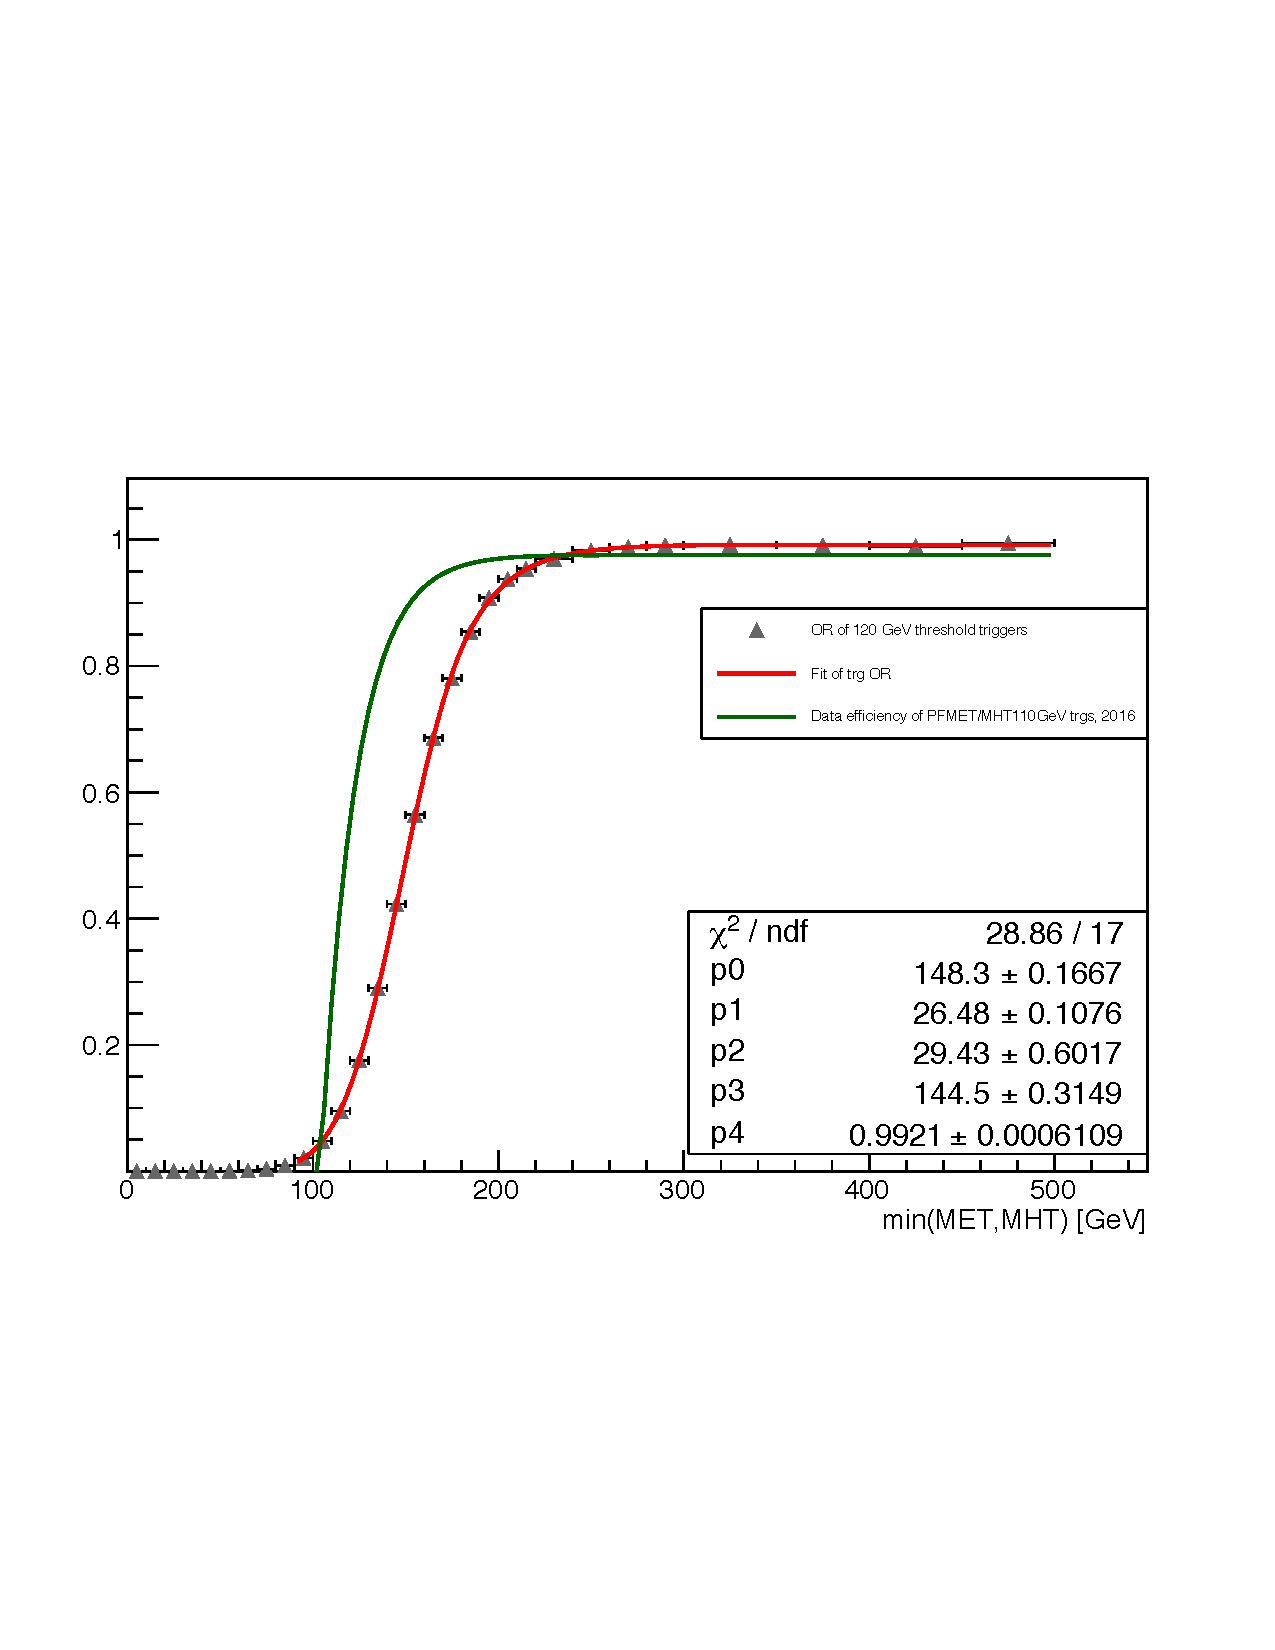
\includegraphics[width=3.75in]{images/2017METTriggersData}
    \caption[Trigger Efficiency for \ZnnHbb\ in 2017 Data]{The trigger efficiency for the \ZnnHbb\ channel as a function of the minimum of the offline MET and MHT measured using the full 2017 SingleElectron primary dataset. The green curve represents the efficiency in 2016 data of the logical \texttt{OR} of analogous triggers used by the 2016 analysis. The red curve represents the efficiency of the logical \texttt{OR} of the triggers used for the 2017 analysis.}
    \label{fig:triggersdata}
\end{figure}

The MET trigger efficiency can also be measured using MC samples to assess the trigger emulation performance. The trigger efficiency curve of the emulated MET triggers is obtained using the same procedure as for data and is shown in Figure \ref{fig:triggersmc}. An efficiency correction is obtained by taking the ratio of the fitted trigger efficiency curve for data to that of simulation and is shown in Figure \ref{fig:triggersunc}. The correction reaches up to 9\% in the ``turn-on'' region of the efficiency curve, but then remains close to unity upon reaching the plateau. The uncertainty of this efficiency correction were determined by the eigenvector decomposition of the covariance matrices of the fitted functions for data and simulation, and those which have non-negligible effects on the shape of the final discriminant or process normalizations are assessed as systematic uncertainties.

\begin{figure}[htbp]
  \centering
    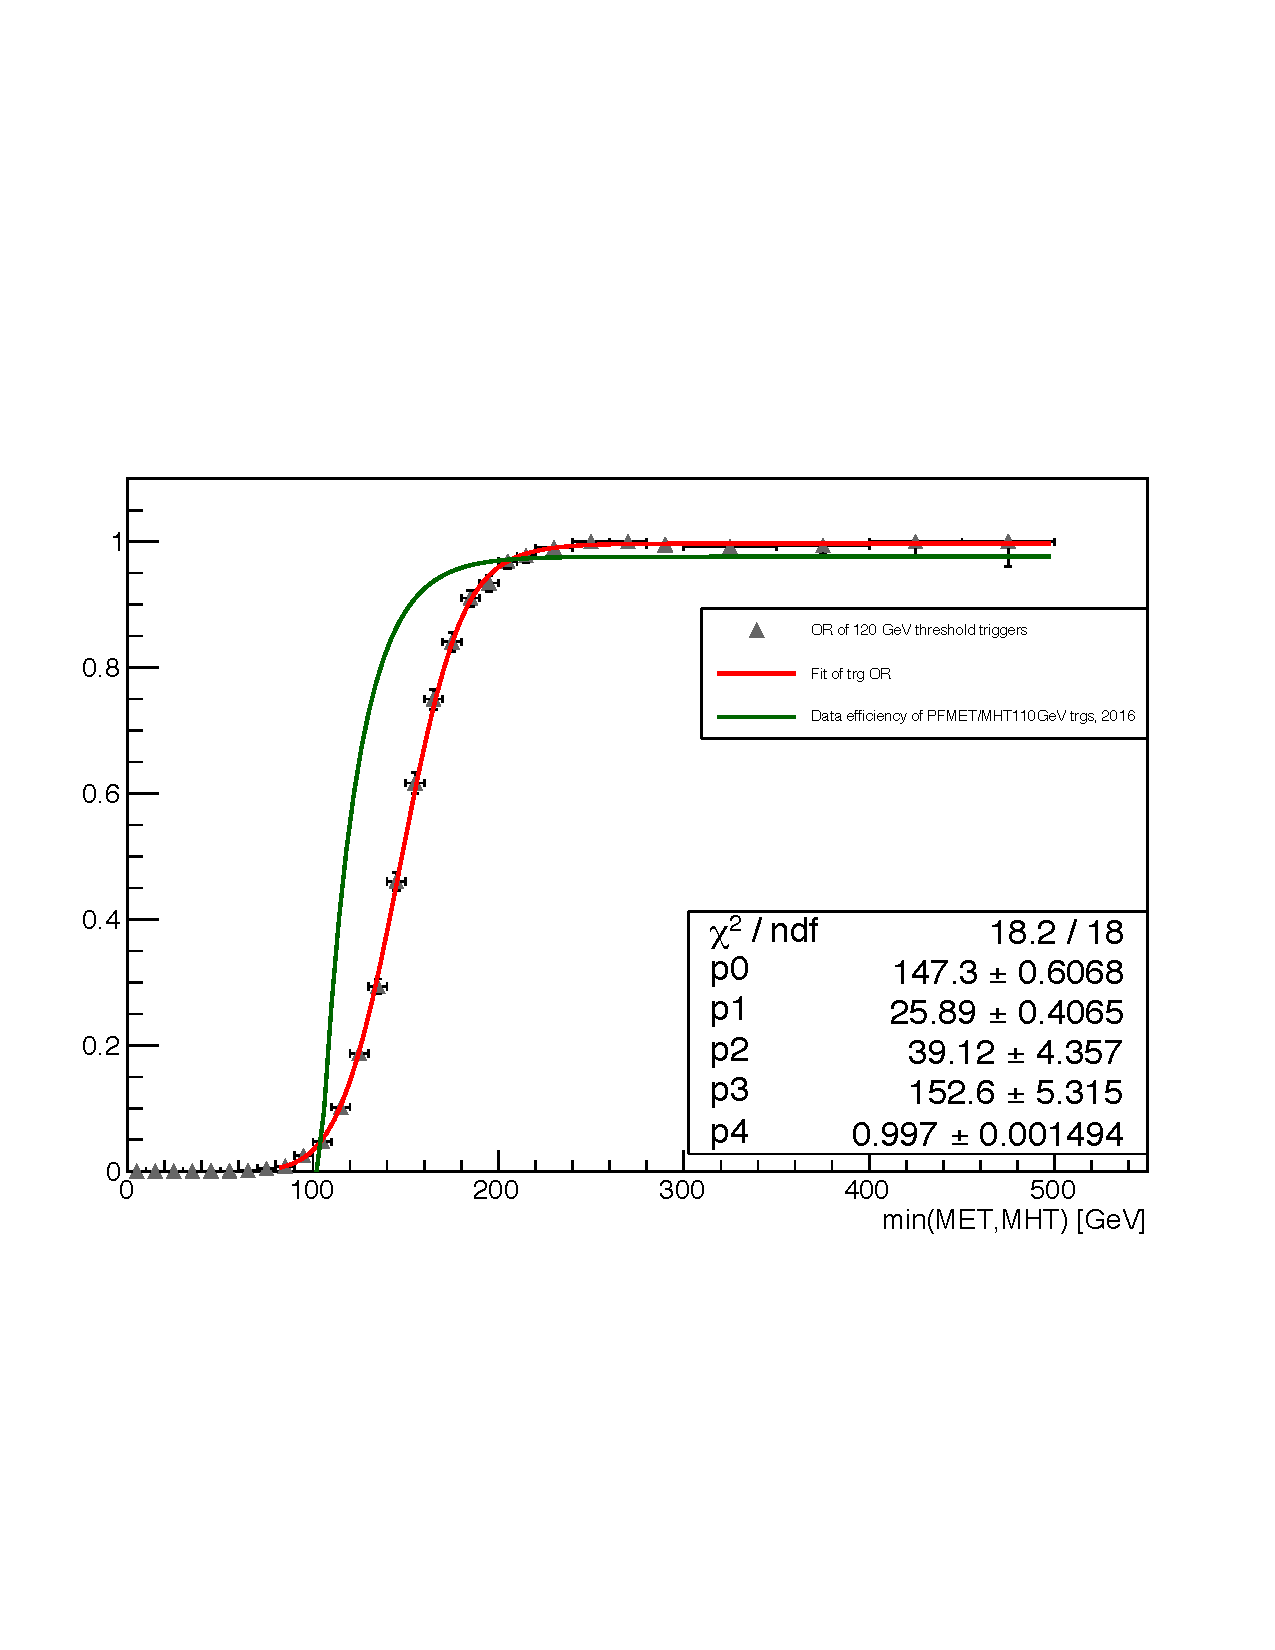
\includegraphics[width=3.75in]{images/2017METTriggersMC}
    \caption[Trigger Efficiency for \ZnnHbb\ in 2017 MC]{The emulated trigger efficiency for the \ZnnHbb\ channel as a function of the minimum of the offline MET and MHT measured using a $\bosW + 3\textrm{-jets}$ Monte-Carlo sample. The green curve represents the efficiency in 2016 data of the logical \texttt{OR} of analogous triggers used by the 2016 analysis. The red curve represents the efficiency of the emulated logical \texttt{OR} of the triggers used for the 2017 analysis.}
    \label{fig:triggersmc}
\end{figure}

\begin{figure}[htbp]
  \centering
  \mbox{
    \subfigure [] {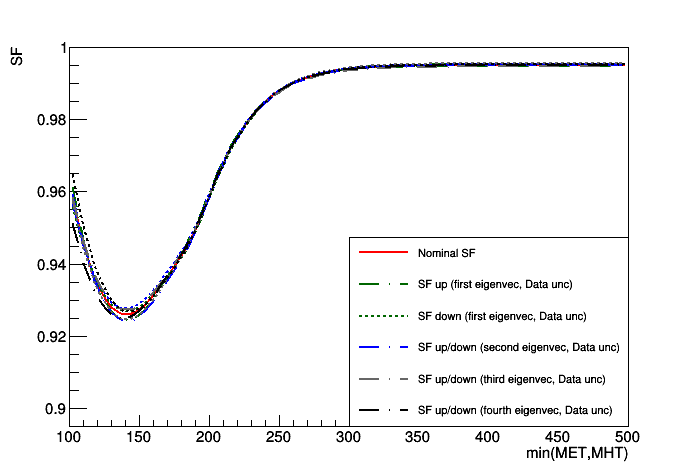
\includegraphics[scale=0.33]{images/metTrigger2017SF_dataunc}} \quad
    \subfigure [] {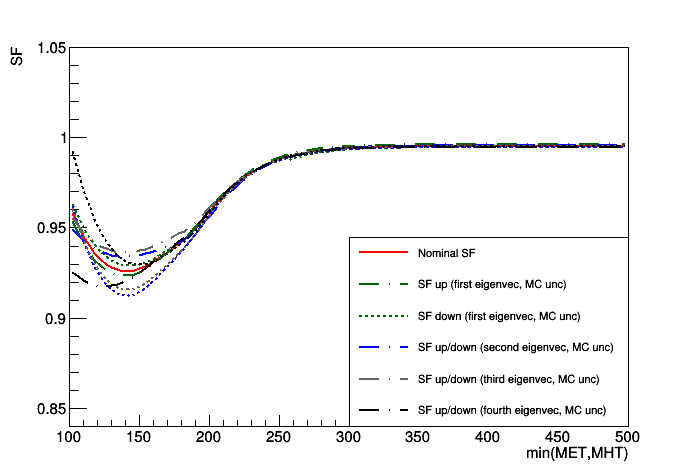
\includegraphics[scale=0.33]{images/metTrigger2017SF_mcunc}} \quad
  }
  \caption[2017 MET Trigger Efficiency Correction for \ZnnHbb]{The MET trigger efficiency correction for the \ZnnHbb\ channel as a function of the minimum of the offline MET and MHT. The red curve represents the nominal correction, while the dotted and dash-dotted curves represent the variations in the correction due to the four leading uncertainties in A) data and B) Monte-Carlo.}
    \label{fig:triggersunc}
\end{figure}

The trigger efficiencies for the other decays channels are similarly handled. The triggers used by the \WlnH\ channel reach efficiencies of approximately 90\% for electrons and 95\% for muons. The triggers used by the \ZllH\ channel reach efficiencies of approximately 96\% for electrons and 91\% for muons.

\subsection{Residual Monte-Carlo Corrections}

Although the MC samples provide realistic simulations of physics processes, discrepancies between the shapes of kinematic distributions in data and MC remain a concern. The presence of such observed differences is not unexpected, given the fixed-order accuracy of and the assumptions made by the event generators. Residual corrections therefore need to be applied to the MC samples to improve the agreement between data and MC for key distributions.

The first such correction addresses the difference between the \pTV\ spectrum in data and the \bosV+jets MC samples. The \pTV\ distribution is harder for simulation than for data because the simulation does not include higher-order electroweak corrections.\cite{EWKCORR} The \bosV+jets samples are therefore reweighted as a function of the \pTV\ to apply the NLO electroweak correction shown in Figure \ref{fig:vjetsewkweight} which accounts for discrepancies of up to 10\% for \pTV\ near 400 \GeV.

\begin{figure}[htbp]
  \centering
    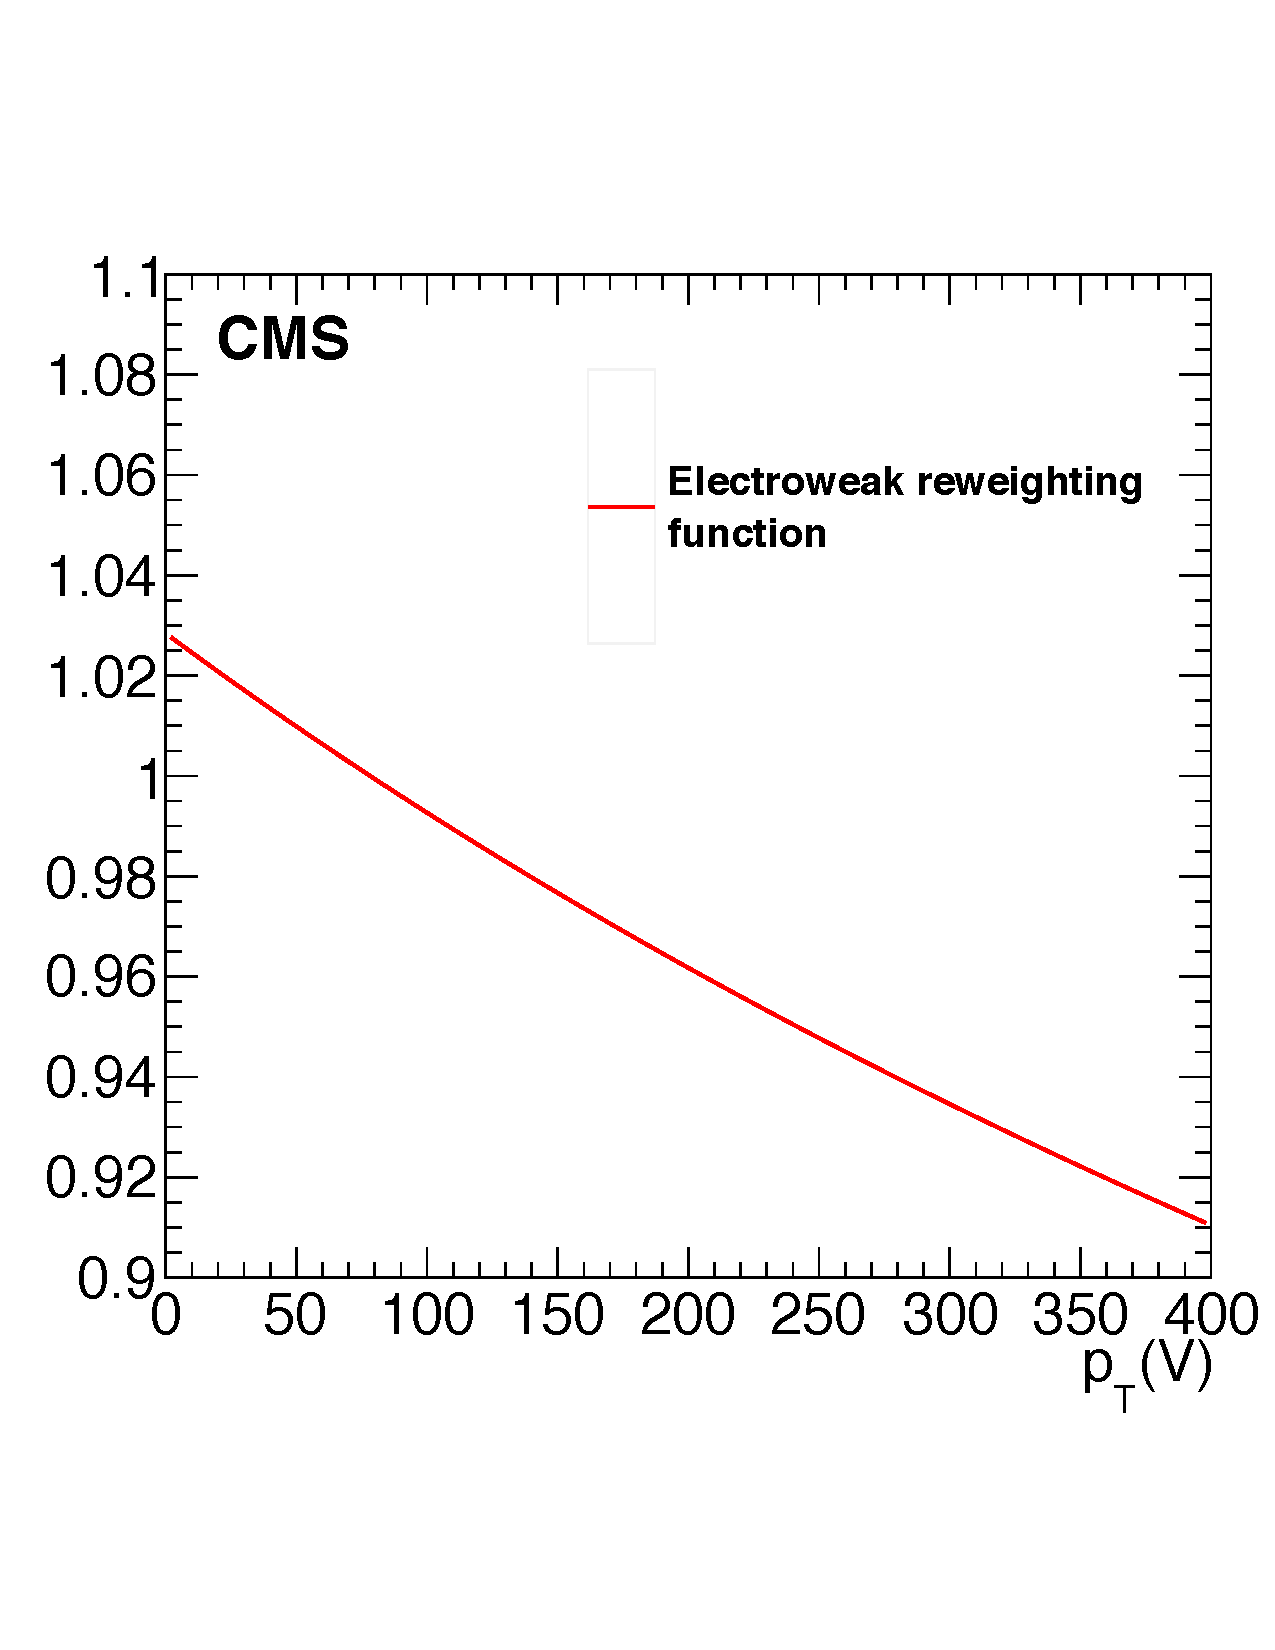
\includegraphics[width=3in]{images/ewk_vjets_correction}
    \caption[2017 \bosV+jets MC Electroweak Correction]{The NLO electroweak correction applied to the \bosV+jets Monte-Carlo samples.}
    \label{fig:vjetsewkweight}
\end{figure}

The second such correction addresses the difference between the \pT\ spectra of the top quarks in data and the $\qrkt\bar{\qrkt}$ MC samples. The \pT\ spectra of top quarks in data are observed to be softer than predicted by the event generators. The $\qrkt\bar{\qrkt}$ samples are therefore reweighted as a function of the top quark \pT\ according to the official recommendation by the CMS experiment.\cite{CMSTTCORR} This correction is only applicable for the \ZnnH\ and \ZllH\ channels, and is superceded by an equivalent reweighting specific to the \WlnH\ channel.

A third correction addresses the discrepancy between the di-jet invariant mass \mjj\ distribution in data and the LO \bosV+jets MC samples. Although NLO \bosV+jets MC samples are readily available and show good agreement with data for the \mjj\ distribution, they are not used by the analysis because their limited statistical power results in an over 10\% decrease in expected sensitivity with respect to the LO \bosV+jets samples. A differential LO-to-NLO correction based on the separation in $\eta$ between the two \qrkb-quark jets from the Higgs boson decay $\Delta\eta(jj)$ is derived as a ratio of the NLO to LO \bosV+jets samples following the procedure outlined in Ref. \cite{CMSVHbbEvidence}. An example of this ratio is shown in Figure \ref{fig:NLOtoLOratio}. These reweighting functions improve the agreement between data and the LO \bosV+jets samples for the \mjj\ and \pTV\ distributions while demonstrating a negligible effect on the remaining distributions. The full reweighting is assessed as a systematic uncertainty.

\begin{figure}[htbp]
  \centering
    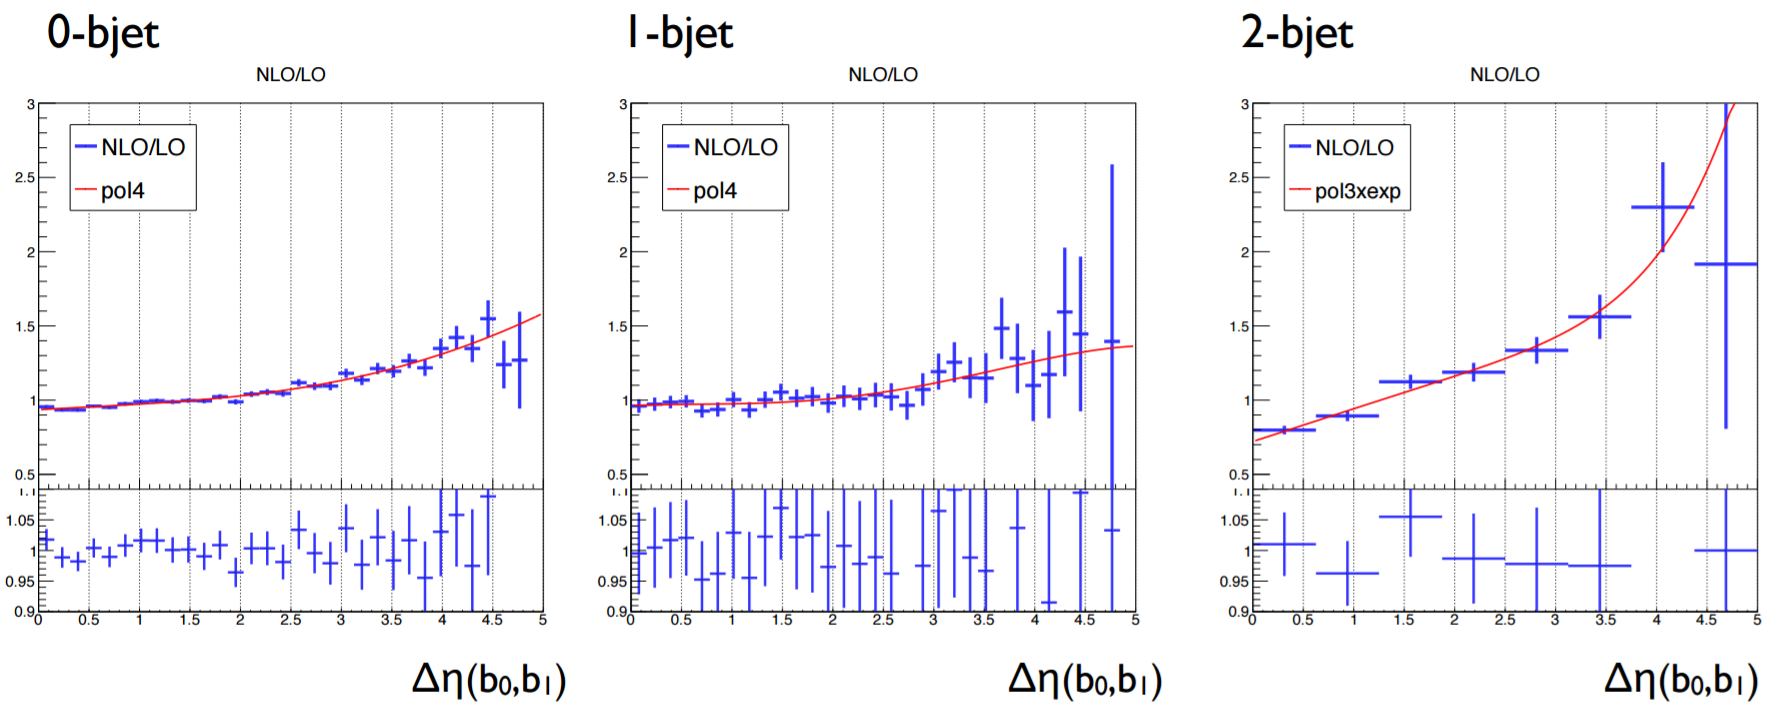
\includegraphics[width=6in]{images/NLOtoLO}
    \caption[NLO to LO Ratio of $\Delta\eta(jj)$ for \bosZ+jets $(\bosZ \rightarrow \ell\bar{\ell})$ Samples]{The ratio of $\Delta\eta(jj)$ between the NLO to LO \bosZ+jets $(\bosZ \rightarrow \ell\bar{\ell})$ Monte-Carlo samples divided into categories based on the number of true \qrkb-jets present.}
    \label{fig:NLOtoLOratio}
\end{figure}

A final correction addresses the downward trend in the data to MC ratio for the \pTV\ distribution that is observed in the control regions of the \WlnH\ channel. A simultaneous fit of the \pTV\ distribution to data in the control regions of the \WlnH\ channel are used to derive independent linear reweighting functions for the $\qrkt\bar{\qrkt}$, \bosW\ with light-flavored jets (\Wlight), and combination of \bosW\ with \qrkb-jets (\Wbb) and single top processes. The relative compositions of the background processes were fixed during the fit and the reweighting preserves the overall normalization. The uncertainties on the fitted slopes of the linear reweighting functions are taken to be the systematic uncertainties of this \pTV\ correction. An uncertainty of 13\% is assessed for the $\qrkt\bar{\qrkt}$ reweighting, while a 6\% uncertainty is assessed for both the \Wlight\ and \Wbb\ and single top combined reweightings. These uncertainties sufficiently cover any perceived discrepancies after all corrections have been applied.

\section{Physics Objects}

The standard physics object candidates reconstructed by the PF algorithm and described in Chapter \ref{reco} are used by the analysis. The identification and selection of electrons, muons, jets, \qrkb-jets, and MET proceeds according to recipes approved and provided by their corresponding Physics Object Group (POG). Recommended working points and corrections are also applied, as well as additional reconstruction techniques developed for the \VHbb\ analysis.

The primary vertex candidates are reconstructed according to the deterministic annealing algorithm.\cite{ITERTRACK} The signal vertex, the primary vertex corresponding to the primary hard interaction which triggered the event, is chosen to be the primary vertex with the largest $\sum \pT^{2}$, where the sum runs over all elementary particles identified at the tracking level, namely track-jets, track-MET, and charged leptons. In addition, displaced tracks originating from the decay of \qrkb-hadrons are associated with to their proper primary vertex to increase the probability of choosing the correct signal vertex, especially for the \ZnnH\ channel which searches for a decay final state with two \qrkb-jets and large MET.

Because of the high instantaneous luminosity and tight bunch crossing timing, the number of reconstructed primary vertices increases with the amount of pileup, or additional proton-proton interactions that may be \textit{in-time}, occurring within the same bunch crossing considered by the event, or \textit{out-of-time}, occurring within the previous or next bunch crossings. The presence of pileup interactions impacts the choice of signal vertex as well as the reconstruction of all other objects by worsening the momentum resolution of jets and, by extension, MET and affecting the calculation of lepton isolation and the performance of \qrkb-taggers. The analysis addresses pileup effects by employing the following approaches:
\begin{itemize}
  \item \textbf{Charged hadronic subtraction (CHS)} is an algorithm integrated with the reconstruction algorithm for PF jets which filters all charged hadrons whose trajectories are incompatible with the primary interaction.
  \item \textbf{FastJet substraction} is an algorithm provided by the \texttt{FastJet}\cite{FASTJET} software package which calculates the average momentum density per unit area due to pileup for each event which is used to decontiminate jet and lepton isolation cones.
\end{itemize}
Finally, to account for observed differences between the pileup distribution in data and MC simulation, the simulated events are reweighted to match the amount of generated pileup. After the effects of pileup have been treated, the agreement between data and simulation is much better, as demonstrated in Figure \ref{fig:rho}.

\begin{figure}[htbp]
  \centering
    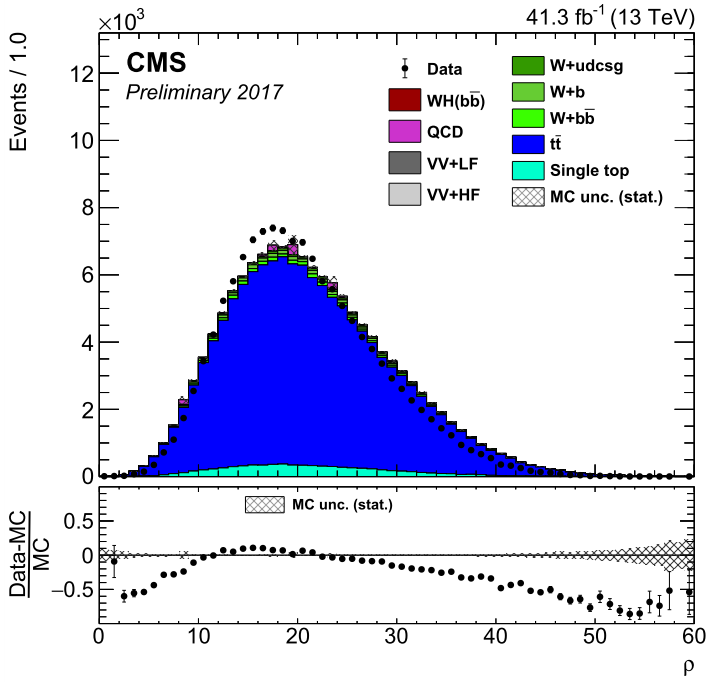
\includegraphics[width=3in]{images/rho}
    \caption[Average Jet Energy Density in 2017 Data]{The distribution of the average jet energy density $\rho$ for 2017 data and simultion in the \qrkt\qrktbar control region of the \WlnH\ channel which is defined in section \ref{CRs}.}
    \label{fig:rho}
\end{figure}

Electrons are reconstructed using the Gaussian-sum filter (GSF) algorithm.\cite{GSFTRACK} The electron candidates are then selected by first applying a loose relative isolation cut of 0.4, after which they must pass tighter identification requirements based on multivariate discriminator thresholds determined by the Electron-Gamma (EGM) POG. Two of the prescribed working points are used:
\begin{itemize}
  \item The loose working point (WP90) achieves an electron selection efficiency of 90\% and is used by the analysis to perform an initial categorization of event candidates for every decay channel as well as to identify the electrons in the \ZeeH\ channel.
  \item The tight working point (WP80) achieves an electron selection efficiency of 80\% and is used to identify electrons in the \WenH\ channel and suppress background.
\end{itemize}
Tn order to reduce the multijet background, the electron isolation cut is specifically tightened to 0.06 for the \WenH\ channel. The \ZeeH\ channel loosened the electron isolation cut to 0.15 because its requirement of two leptons in the final state virtually eliminates all multijet background for that channel, allowing it to increase its signal efficiency at little cost.

Muons are reconstructed using tracker muon tracks and global muon tracks identified by the PF algorithm. The muon candidates are also selected by first applying a loose relative isolation cut of 0.4, after which they are required to pass tighter criteria proposed by the Muon POG which are based on the results of the global muon track fit and information from the tracker which are used to determine if it the muon is prompt. The \WmnH\ channel tightened the muon isolation cut to 0.06, which by chance is the same value used by the \WenH\ channel for the electron isolation cut, in order to remove data excesses in the poorly modelled tails of the isolation distribution. The \ZmmH\ channel loosened the muon isolation cut to 0.12 for same reasons the \ZeeH\ channel loosened its electron isolation cut.

Jets are reconstructed using the anti-$k_{T}$ jet clustering algorithm\cite{ANTIKT} to cluster together PF candidates with a radius parameter of $R = 0.4$ to form so-called ``AK4'' jets. The jet energy scale (JES) corrections recommended by the Jet/MET (JME) POG and derived for 2017 data and simulation were applied to calibrate the energy of the jets. The jet energies are also smeared in simulation in order for the resolution in simulation to match the resolution in data. A loose jet identification is applied that rejects misreconstructed candidates due to detector noise or contamination from pileup energy. Jets overlapping a preselected electron or muon are discarded, and jets which are outside of the tracker acceptance of $\left| \eta \right| < 2.5$ are not considered by the analysis.

The identification of jets initiated by the hadronization of \qrkb-quarks is performed using the Deep Combined Secondary Vertex (DeepCSV)\cite{CMSBTAG} \qrkb-tagging algorithm. The DeepCSV tagger uses as its discriminator a neural network classifier which takes as input information from secondary vertices and track impact parameters associated with a jet in an event and outputs five continuous values that are interpreted to be the probabilities that the jet belongs to one of five different possible hadronization scenarios described in section \ref{btagging}. In the context of this analysis, the DeepCSV score refers to the summed probability that a jet originated from a \qrkb-quark or two \qrkb-quarks, as the Higgs boson will be reconstructed from a compatible pair of \qrkb-jet candidates. The \qrkb-Tagging and Vertexing (BTV) POG recommends three working points, shown in Table \ref{tbl:deepcsvwp}, which trade off between \qrkb-tagging efficiency and misidentification rate.

\begin{table}[htbp]
  \caption[2017 DeepCSV Working Points]{The 2017 \qrkb-tagging working points defined for the DeepCSV algorithm, along with their associated misidentification rates.\cite{CMSBTAG}}
  \label{tbl:deepcsvwp}
  \begin{tabularx}{6.5in}{XXr}
    \hline
    Working Point & DeepCSV Score & Misidentification Rate \\
    \hline
    Loose         & 0.1522        & 10.0\%                 \\
    Medium        & 0.4941        & 1.0\%                  \\
    Tight         & 0.8001        & 0.1\%                  \\
    \hline
  \end{tabularx}
\end{table}

Observed discrepancies in the \qrkb-tagging efficiency between data and simulation are addressed by calibrating the DeepCSV discriminator values using a tag-and-probe (TnP) approach such that the the DeepCSV distribution for jets in simulation matches the distribution observed in data control regions. The binned distribution of the probe jets in data is compared to the expected distrbution from simulation and an iterative procedure scales the content of each bin to match while preserving the expected proportions of light and heavy flavor jets. The procedure itself is carried out in bins of \pT\ and $\eta$. The ratio of the scaled distribution in simulation to the original distribution in simulation defines a per jet weight $w_{j}$ which is function of DeepCSV and parameterized by the jet \pT, $\eta$, and flavor. For an event with $N_{\mathrm{jets}}$, the product of the weights for each jet $j$ defines an overall \qrkb-tag calibration weight
\begin{equation}
  w_{\qrkb\text{-}\mathrm{tag}} = \prod_{j=1}^{N_{\mathrm{jets}}} w_{j} \left( \mathrm{DeepCSV}_{j} | p_{\mathrm{T}j}, \eta_{j}, \mathrm{flavor}_{j} \right).
  \label{eq:btagweight}
\end{equation}

The missing transverse momentum $vec{p}_{\mathrm{T}}^{\mathrm{miss}}$ is reconstructed as the negative vectorial sum of the transverse momentum of all PF objects identified in the event. The magnitude of $vec{p}_{\mathrm{T}}^{\mathrm{miss}}$ is the missing transverse energy \pTmiss, or colloquially MET. A Type-I correction, where the JES corrections are applied to the PF jets which enter the vectorial sum, is applied to calibrate the MET. The jet smearing is also propagated to the MET calculation to more realistically match the resolution of the MET in data. Finally, events with large MET caused by spurious detector noise are rejected by applying the standard set of MET filters recommended by the JetMET POG. In addition to the MET, the missing hadronic transverse energy MHT is also used by the \ZnnH\ channel, which is defined as the magnitude of the missing hadronic transverse momentum, or the negative vectorial sum of the transverse momenta of only jets with $\pT > 30\ \GeV$ and $\left| \eta \right| < 2.4$.

Aside from the vector boson and Higgs boson decays, additional hadronic activity is expected to be low for signal events. The remaining activity is expected to be soft, and so any low \pT\ tracks originating from the signal vertex but not associated with the vector boson or Higgs boson candidates are used to reconstruct the ``soft activity''. These tracks are then clustered into AK4 ``soft-track jets'' which have been demonstrated to capably reconstruct the hadronization of very low energy partons.\cite{CMSTRACKJETS} To further separate signal from background, the \VHbb\ analysis defines and uses the quantity SA5, which is the number of soft-track jets in the event with $\pT > 5\ \GeV$.

\subsection{Vector Boson Candidate}

For the \ZnnH\ channel, the vector boson is simply reconstructed from large MET because the \bosZ\ decays invisibly to a pair of neutrinos. Candidate \ZnnH\ events are required to have $\mathrm{MET} > 150\ \GeV$, and the transverse momentum of the reconstructed \bosZ\ candidate is defined as $\pT(\bosZ) = \min \left( \mathrm{MET}, \mathrm{MHT} \right)$. In order to remove observed discrepancies between the data and simulation in the turn-on region of the MET trigger efficiency curve, the analysis of the \ZnnH\ channel only considers events with $\pT(\bosZ) > 170 \GeV$.

For the remaining channels, the vector boson reconstruction involves the selection and identification of isolated leptons. For the \ZllH\ channels, the \bosZ\ boson is reconstructed from pairs of isolated electrons or muons which have a dilepton invariant mass $m(\ell\ell)$ within the range $75\ \GeV < m(\ell\ell) < 105\ GeV$ which covers the on and off-shell decays of the \bosZ\ boson. Separate analyses of the \ZllH\ channels are then performed for \bosZ\ boson candidates in a low \pT\ category ($50\ \GeV < \pT(\bosZ) < 150\ \GeV$) and high \pT\ category ($\pT(\bosZ) > 150\ \GeV$). For the \WlnH\ channels, the \bosW\ boson is reconstructed from a single isolated electron or muon and the MET and the transverse momentum and transverse mass of the \bosW\ boson candidate is defined as
\begin{equation}
  \pT(\bosW) = \sqrt{\left( \mathrm{MET}_{x} + p_{x}^{\ell} \right)^{2} + \left( \mathrm{MET}_{y} + p_{y}^{\ell} \right)^{2}}
  \label{eq:WlnWpT}
\end{equation}
and
\begin{equation}
  m_{T}(\bosW) = \sqrt{\left( \mathrm{MET}_{x} + p_{\mathrm{T}}^{\ell} \right)^{2} - \pT(\bosW)^{2}},
  \label{eq:WlnWmT}
\end{equation}
where $p^{\ell}$ is the four-momentum of the isolated lepton.

\subsection{Higgs Boson Candidate}

For all decay channels, the Higgs boson is most efficienctly reconstructed using the pair of \qrkb-jets with the largest DeepCSV score per event, where the leading \qrkb-jet is required to pass the tight working point cut for all channels except \ZllH\ and the subleading \qrkb-jet is required to pass the loose working point. Because the identification of the Higgs boson candidate is crucial to the analysis, advanced techniques are used to improve the dijet invariant mass resolution. The application of a \qrkb-jet energy regression, a kinematic fit in the \ZllH\ channel, and a recovery of final state radiation (FSR) results in a channel-dependent improvement of 10-23\% for the mass resolution.

The \qrkb-jet energy regression is used to correct the energies of \qrkb-jets by providing an accurate estimate of the true \qrkb-jet energy and resolution. The multitarget regression is modelled using a neural network implemented using the \texttt{Keras}\cite{KERAS} neural network framework with \texttt{Tensorflow}\cite{TENSORFLOW} as the backend. There are 43 input features based on the \qrkb-jet kinematics, pileup in the event, leading tracks in the \qrkb-jet, soft-lepton tracks in the \qrkb-jet, secondary vertex candidates, and \qrkb-jet energy fractions carried by electromagnetic, charged, and neutral constituents in five rings of $\Delta R$ within the jet cone. The architecture of the neural network model uses six hidden layers with the number of nodes in each layer being 1024, 1024, 1024, 512, 256, and 128, respectively. The hidden layer nodes are leaky rectified linear units (Leaky ReLU)\cite{RELU} with a slope of $\beta = 0.2$ for the negative part of its argument:
\begin{equation}
  f(x) = \begin{cases}
           x, & \mathrm{ if x > 0} \\
           \beta x, & \mathrm{ otherwise} \\
         \end{cases}
       = \begin{cases}                                                                                                                               
           x, & \mathrm{ if x > 0} \\
           0.2 x, & \mathrm{ otherwise} \\
         \end{cases}.
  \label{eq:leakyrelu}
\end{equation}
Batch-normalization\cite{BATCHNORM} and dropout\cite{DROPOUT} with a probability of 0.1 are applied to the outputs of each hidden layer to increase the training speed and regularize the model. The output layer consists of three linear nodes, one of which is trained to estimate the jet energy correction while the others are trained to estimate the jet energy resolution at 25\% and 75\% quantiles. A composite loss function is used, which is taken to be the sum of the Huber loss\cite{HUBER} for the jet energy correction task and two asymmetrically-weighted quantile losses for the jet energy resolution tasks. The training was performed with stochastic gradient descent using adaptive moment estimation, or the Adam optimizer.\cite{ADAM} The model hyperparameters were optimized by taking the best performing random model out of 50 trials sampled from a discrete grid. By calibrating the \qrkb-jets energies using the corrections obtained by the regression, channel-dependent improvements of 10-23\% for the mass resolution are observed, with the improvements to the \ZllH\ channel shown in Figure \ref{fig:bjetreg_perf}.

\begin{figure}[htbp]
  \centering
  \mbox{
    \subfigure [] {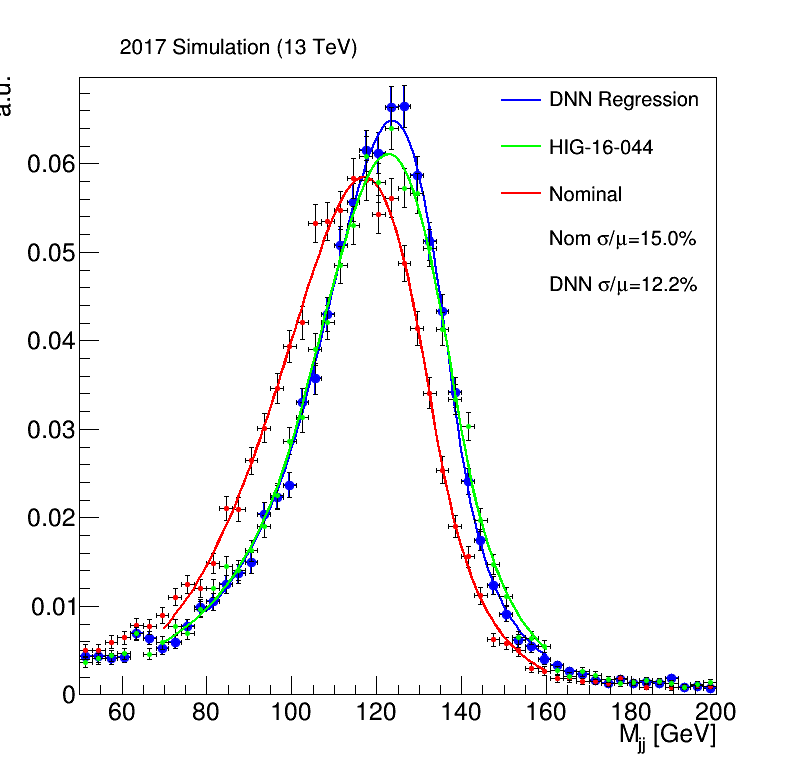
\includegraphics[scale=0.28]{images/RegressionPerformance_nolep_Zll_2017}} \qquad
    \subfigure [] {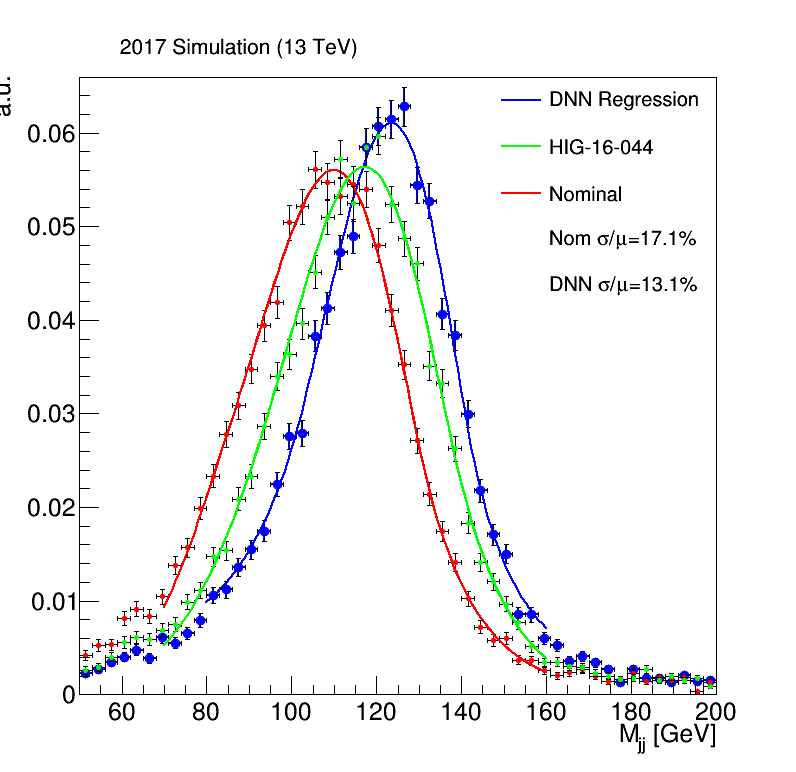
\includegraphics[scale=0.28]{images/RegressionPerformance_semilep_Zll_2017}} \qquad
  }
  \caption[Performance of \qrkb-jet Energy Regression]{The dijet invariant mass distribution of the \ZllH\ channel before (red) and after the \qrkb-jet energy regression is applied for A) \qrkb-jets which do not contain leptons and B) \qrkb-jets which contain leptons from semi-leptonic decays of \qrkb-hadrons. The artificial neural network based regression (blue) used by the 2017 analysis outperforms the boosted decision tree based regression (green) used by the 2016 analysis.}
    \label{fig:bjetreg_perf}
\end{figure}

\begin{figure}[htbp]
  \centering
  \mbox{
    \subfigure [] {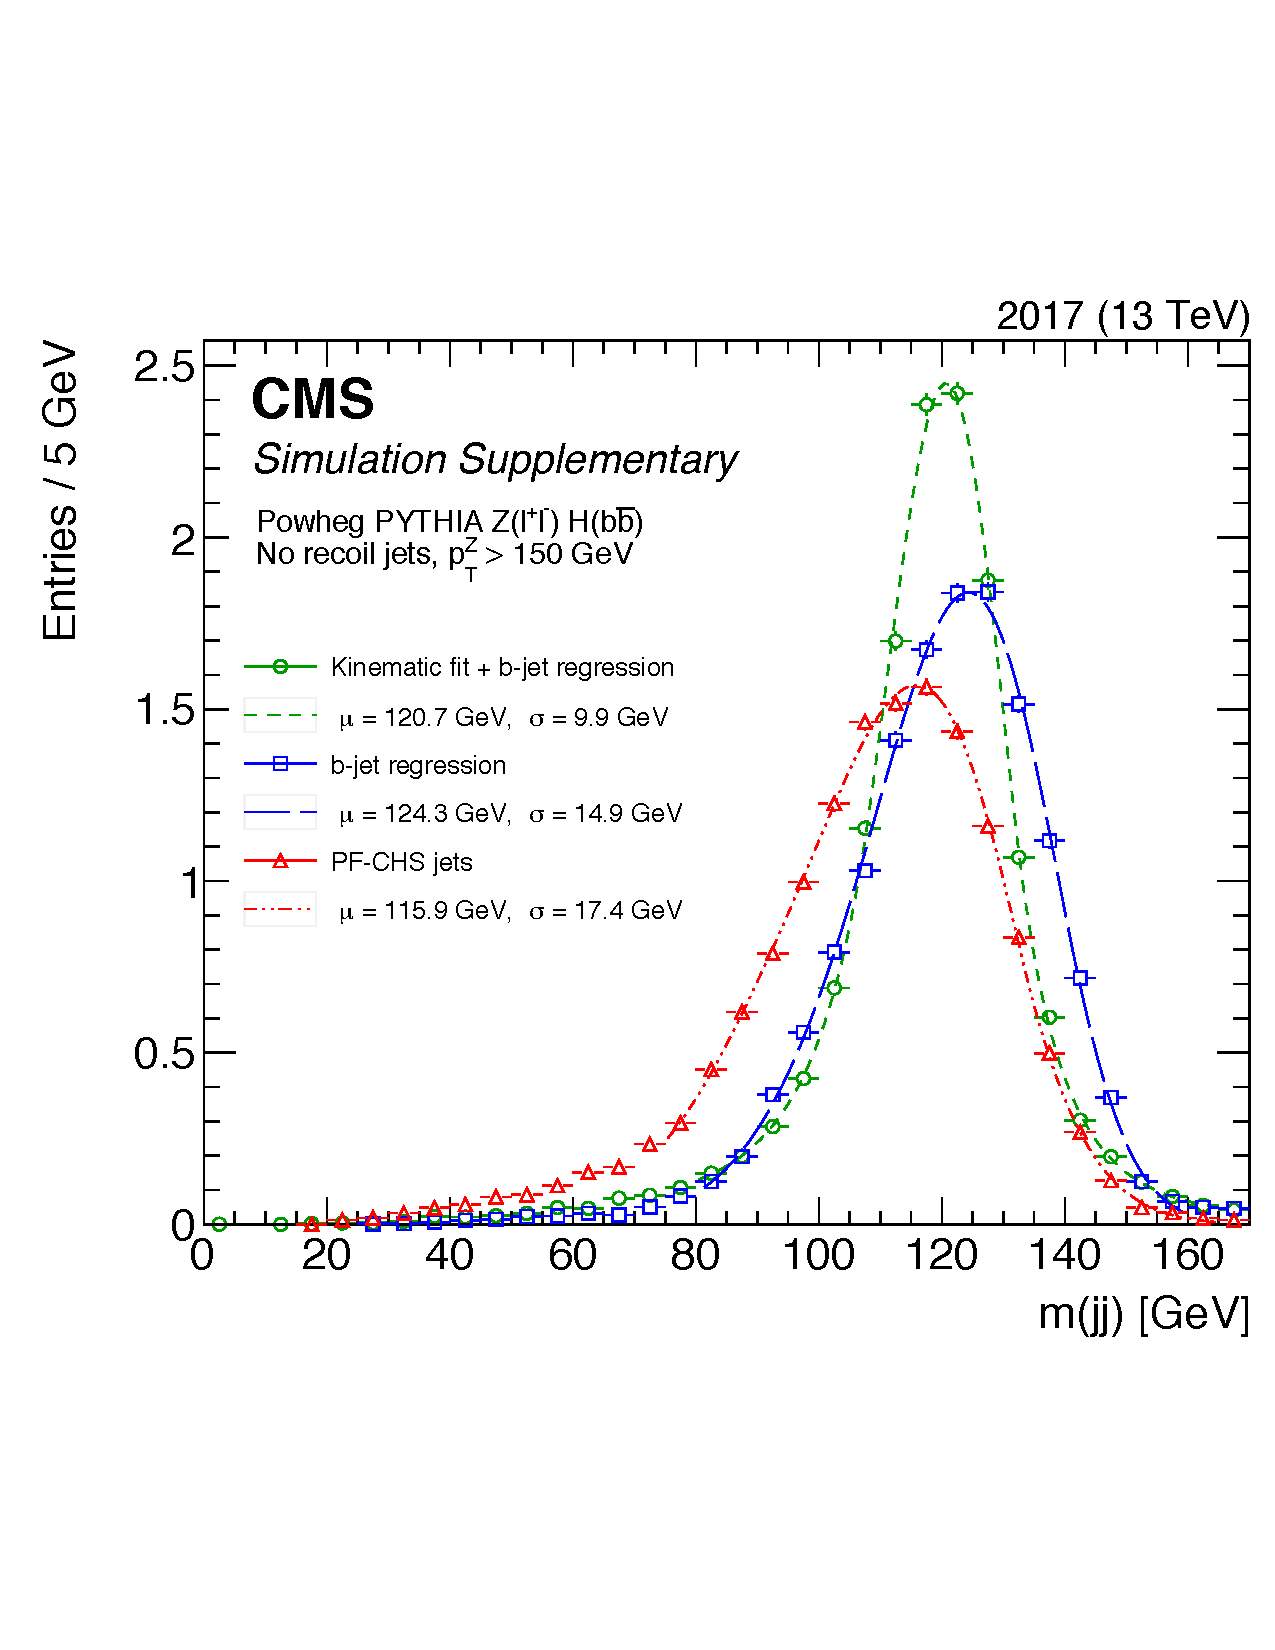
\includegraphics[scale=0.37]{images/CMS-HIG-18-016_Figure-aux_001-a}} \quad
    \subfigure [] {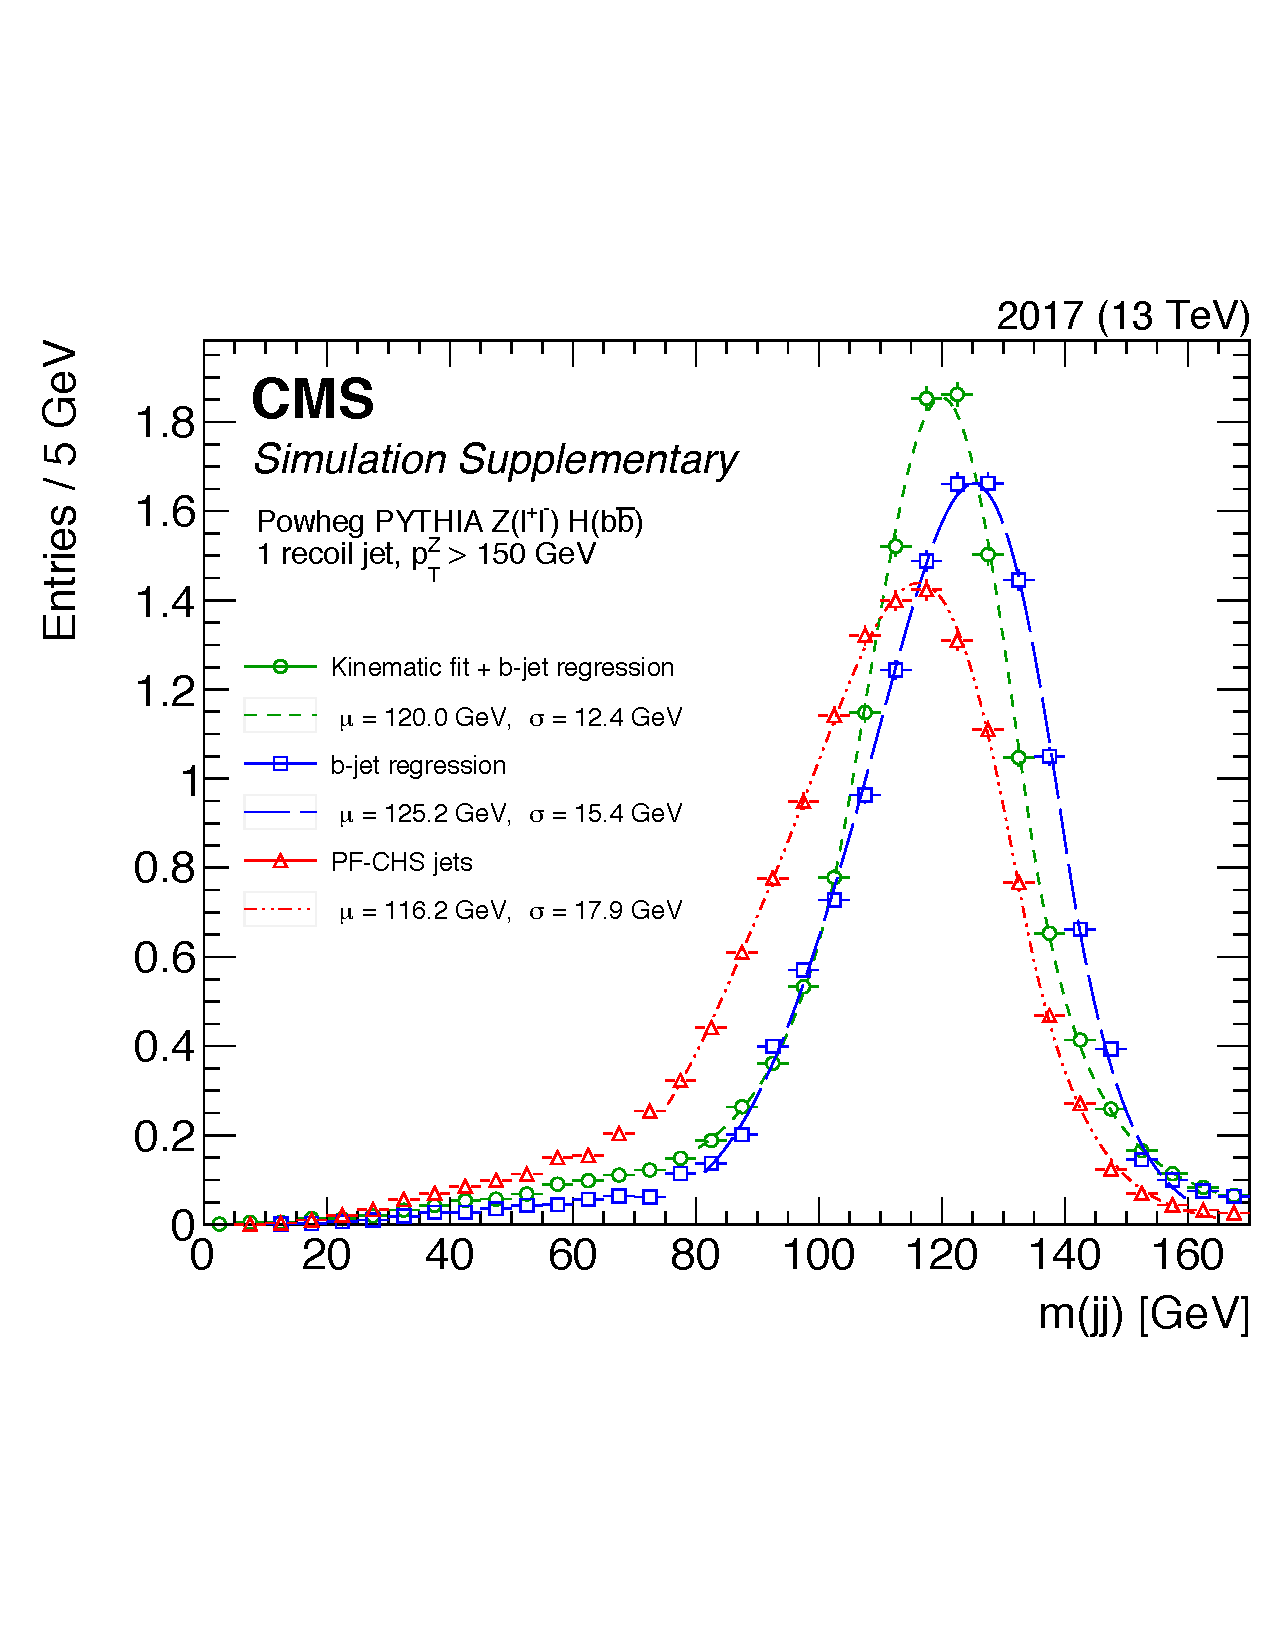
\includegraphics[scale=0.37]{images/CMS-HIG-18-016_Figure-aux_001-b}} \quad
  }
  \caption[Performance of \ZllH\ Kinematic Fit]{The dijet invariant mass distribution of the \ZllH\ channel before (red) and after the \qrkb-jet energy regression corrections (blue) and the kinematic fit (green) are applied for A) events without a recoiling jet and B) events with a single recoiling jet.}
    \label{fig:kinfit_perf}
\end{figure}

The kinematic fit is specific to the \ZllH\ channel because its events have no genuine MET, thereby admitting a unique kinematic constraint which may be exploited to improve the dijet invariant mass resolution. The \texttt{PhysicsTools/KinFitter} package distributed with CMSSW is used to perform the fit, which consists of first constraining the dilepton system to the \bosZ\ boson mass and then constraining the dilepton-dijet system in the transverse plane, all within uncertainties. This balancing of the dilepton and dijet systems also considers a recoil vector to account for jets caused by initial state radiation (ISR). The kinematic fit further improves the dijet invariant mass resolution in the \ZllH\ channel by at least 20\% on top of the \qrkb-jet energy regression, as shown in Figure \ref{fig:kinfit_perf}.

Although a small effect, the final state partons can emit FSR radiation that is collinear to the direction of the \qrkb-jet. In order to recover FSR belonging to the Higgs boson candidates, the four-vectors of soft jets which lie within a cone of $\Delta R <0.8$ around either of the candidate \qrkb-jets used to reconstruct the Higgs boson are added vectorially to the Higgs boson candidate. The FSR recovery results in a channel-dependent improvement of 1-5\% for the dijet invariant mass resolution.

\section{Event Selection}

The analysis applies a channel-dependent event selection in order to maximize the signal purity while reducing the level of background. These selections are primarily motivated by the final state topology of signal process. The \VHbb\ decay considered by the analysis features a leptonically decaying vector boson that recoils away from a pair of \qrkb-jets in the final state. The vector boson candidate and dijet system are therefore expected to be back-to-back in the transverse plane, such that the difference in azimuthal angle between them peaks at $\pi$. Because the invariant mass of the dijet system is expected to be compatible with the mass of the Higgs boson in the range $100\ \GeV < m_{\bosH} < 150\ \GeV$, the \pT\ distributions of the Higgs jet candidates are expected to peak at roughly $m_{\bosH}/2$. Additional activity in the form of isolated leptons which do not originate from the vector boson candidate and soft hadrons are expected to be low.

The event preselections are further refined by considering the final state topologies of the background processes. The \bosV+jets process is the dominant background for all decay channels because it features a true \bosW\ or \bosZ\ boson and one or more jets. Due to its large cross section and similarity to the signal topology, this is the dominant background for all decay channels. It is not entirely irreducible, as detailed comparisons of the final state reveal differences from the signal in terms of the \pT\ distribution of the vector boson, which is typically softer than for signal, and the dijet invariant mass distribution, which falls more sharply. In addition, the majority of these jets are light jets which can be rejected by selecting Higgs jet candidates from those jets which pass the DeepCSV working points.

The \qrkt\qrktbar+jets background process is a dominant background for the \WlnH\ channel. The preferential decay of the top quark to a \bosW\ boson and a \qrkb-quark results in a final state with up to two genuine \bosW\ bosons, either of which may decay leptonically, and at least two \qrkb-jets. However, \qrkt\qrktbar\ background events typically present a higher jet multiplicity, given that one of the \bosW\ bosons may decay hadronically, and a broader distribution for the difference in azimuthal angle between the vector boson candidate and dijet system. The single top background process is irreducible but only represents approximately 10-20\% of the background composition in the \WlnH\ channel, and even less for the other decay channels, due to its smaller cross section.

The Standard Model (SM) diboson production (\bosW\bosW, \bosW\bosZ, \bosZ\bosZ) processes are also important to consider. Because one of the vector bosons can decay leptonically and the other hadronically, their final state topologies mimic that of the signal processes and produces a peak in the dijet invariant mass distribution that is within a few standard deviations of the Higgs mass peak. As this is another irreducible background, diboson events can only be rejected by having a good dijet invariant mass resolution that enables the separation of the diboson and Higgs mass peaks. Incidentally, the properties that make the diboson background difficult to handle also enable it to serve as a ``standard candle'' for the analysis by providing a well-understood SM process with which to validate the analysis strategy. 

\subsection{Signal Regions}

For each decay channel, a signal region is defined based on a selection that reduces the background contamination. The simulated events in the signal region are reserved for the training and validation of the classifier model used to discriminate signal from background, as well as the final statistical analysis, while the data events in the signal region remain blinded until all validation checks have been satisfied. The cuts used to define the signal regions of each decay channel are listed in Table \ref{tbl:signalregions}.

\begin{table}[htbp]
  \caption[Signal Region Definitions for the 2017 \VHbb\ Analysis]{The cuts defining the signal regions of the decay channels for the \VHbb\ analysis. The values of the kinematic quantities are quoted in \GeV\ and the values of the differences in azimuthal angle are quoted in radians. For the \WlnH\ column, the two values for $\pT^{\ell}$ and Tightened Lepton Isolation are applicable for the \WmnH\ and \WenH\ channels, respectively. For the \ZllH\ column, the values for $\pT(\bosV)$ denote the low and high $\pT(\bosV)$ analysis categories, respective.}
  \label{tbl:signalregions}
  \begin{tabularx}{6.5in}{XXXX}
    \hline
    Variable                              & \ZnnH       & \WlnH        & \ZllH             \\
    \hline
    $\pT(\bosV)$                          & $>170$      & $>150$       & $[50, 150], >150$ \\
    $m(\ell\ell)$                         & --          & --           & $[75, 105]$       \\
    $\pT^{\ell}$                          & --          & $>25, >30$   & $>20$             \\
    $\pT(jj)$                             & $>120$      & $>100$       & --                \\
    $m(jj)$                               & $[60, 160]$ & $[90, 150]$  & $[90, 150]$       \\
    \pTjmax                               & $>60$       & $>25$        & $>20$             \\
    \pTjmin                               & $>35$       & $>25$        & $>20$             \\
    \btagmax                              & $>$ Tight   & $>$ Tight    & $>$ Loose         \\
    \btagmin                              & $>$ Loose   & $>$ Loose    & $>$ Loose         \\
    $N_{\mathrm{j}}^{\mathrm{add}}$       & $<2$        & $<2$         & --                \\
    $N_{\mathrm{\ell}}^{\mathrm{add}}$    & $=0$        & $=0$         & --                \\
    \pTmiss                               & $>170$      & --           & --                \\
    $\mathrm{Anti\text{-}QCD}$            & Yes         & --           & --                \\
    $| \Delta\phi(\bosV, \bosH) |$        & $>2.0$      & $>2.5$       & $>2.5$            \\
    $| \Delta\phi(\pTmiss, \pTmisstrk) |$ & $<0.5$      & --           & --                \\
    $| \Delta\phi(\pTmiss, \ell) |$       & --          & $<2.0$       & --                \\
    Lepton Isolation                      & --          & 0.06, 0.06   & --                \\
    \hline
  \end{tabularx}
\end{table}

The analysis of the \ZnnH\ channel is performed in the region of phase space where the transverse momentum of the vector boson $\pT(\bosV)$, which is equivalent to the \pTmiss\ for this signal process, is greater than 170 \GeV\ due to concerns of data to simulation disagreement in the regions in and below the region of the trigger turn-on. This high MET requirement also helps to ``boost'' the events considered by the analysis, which offers a better signal-to-background ratio because the $\pT(\bosV)$ distribution is harder for signal than it is for background. The boosted topology is further reinforced by requiring the transverse momentum of the dijet system $\pT(jj)$ to be greater than 120 \GeV\ and the difference in azimuthal angle between the MET and the dijet system $| \Delta\phi(\bosV, \bosH) |$ to be greater than 2.

The dijet invariant mass $m(jj)$ window is chosen to range from 60 \GeV\ to 160 \GeV, which is wider than for the other decay channels in order to recover background statistics lost by the aggressive thresholds placed on the transverse momenta of the Higgs jet candidates. For the Higgs jet candidate pairs, the \qrkb-jet with the greater DeepCSV score is denoted by \btagmax\ and the lesser by \btagmin, while the larger \qrkb-jet transverse momentum is denoted by \pTjmax\ and the smaller by \pTjmin. The \ZnnH\ analysis places large, asymmetric cuts on \pTjmax\ and \pTjmin\ because of an observed reduction of multijet background.

The number of additional jets $N_{\mathrm{j}}^{\mathrm{add}}$ is at most one and the number of additional leptons $N_{\mathrm{\ell}}^{\mathrm{add}}$ must be zero in order to reject \qrkt\qrktbar\ and multijet backgrounds which have large jet multiplicities and leptons in the final state. The difference in azimuthal angle between the MET and tracker MET $\left| \Delta\phi(\pTmiss, \pTmisstrk) \right|$ is chosen to be less than 0.5 as the direction of the tracker MET is expected to be close to the direction of true MET, given that the \bosZ\ decay does not produce charged leptons. Finally, the Anti-QCD cut is used to strongly reject the multijet background in the \ZnnH\ channel while mainitaining high signal efficiency. The cut is placed on the minimum of the set of differences in azimuthal angle between each jet in an event with $\pT > 30\ \GeV$ and the MET. By requiring this minimum difference to be greater than 0.5, events with fake MET produced by the mismeasurement of jet \pT are removed from the analysis, with approximately 93\% multijet background rejection at 96\% signal efficiency in simulation. The remaining variables which involve leptons are not applicable to the \ZnnH\ channel.

\subsection{Background Control Regions} \label{CRs}

For each decay channel, several control regions are defined by inverting and modifying signal region cuts to produce mutually exclusive samples that are enriched in specific background processes and orthogonal to the signal region. The control regions are used by the analysis to validate the agreement of MC simulation to data and to determine the normalization of key background processes with minimal extrapolation uncertainties during the final statistical analysis. A diagram summarizing the design of the control regions is show in Figure \ref{fig:controlregiondef}.

\begin{figure}[htbp]
  \centering
    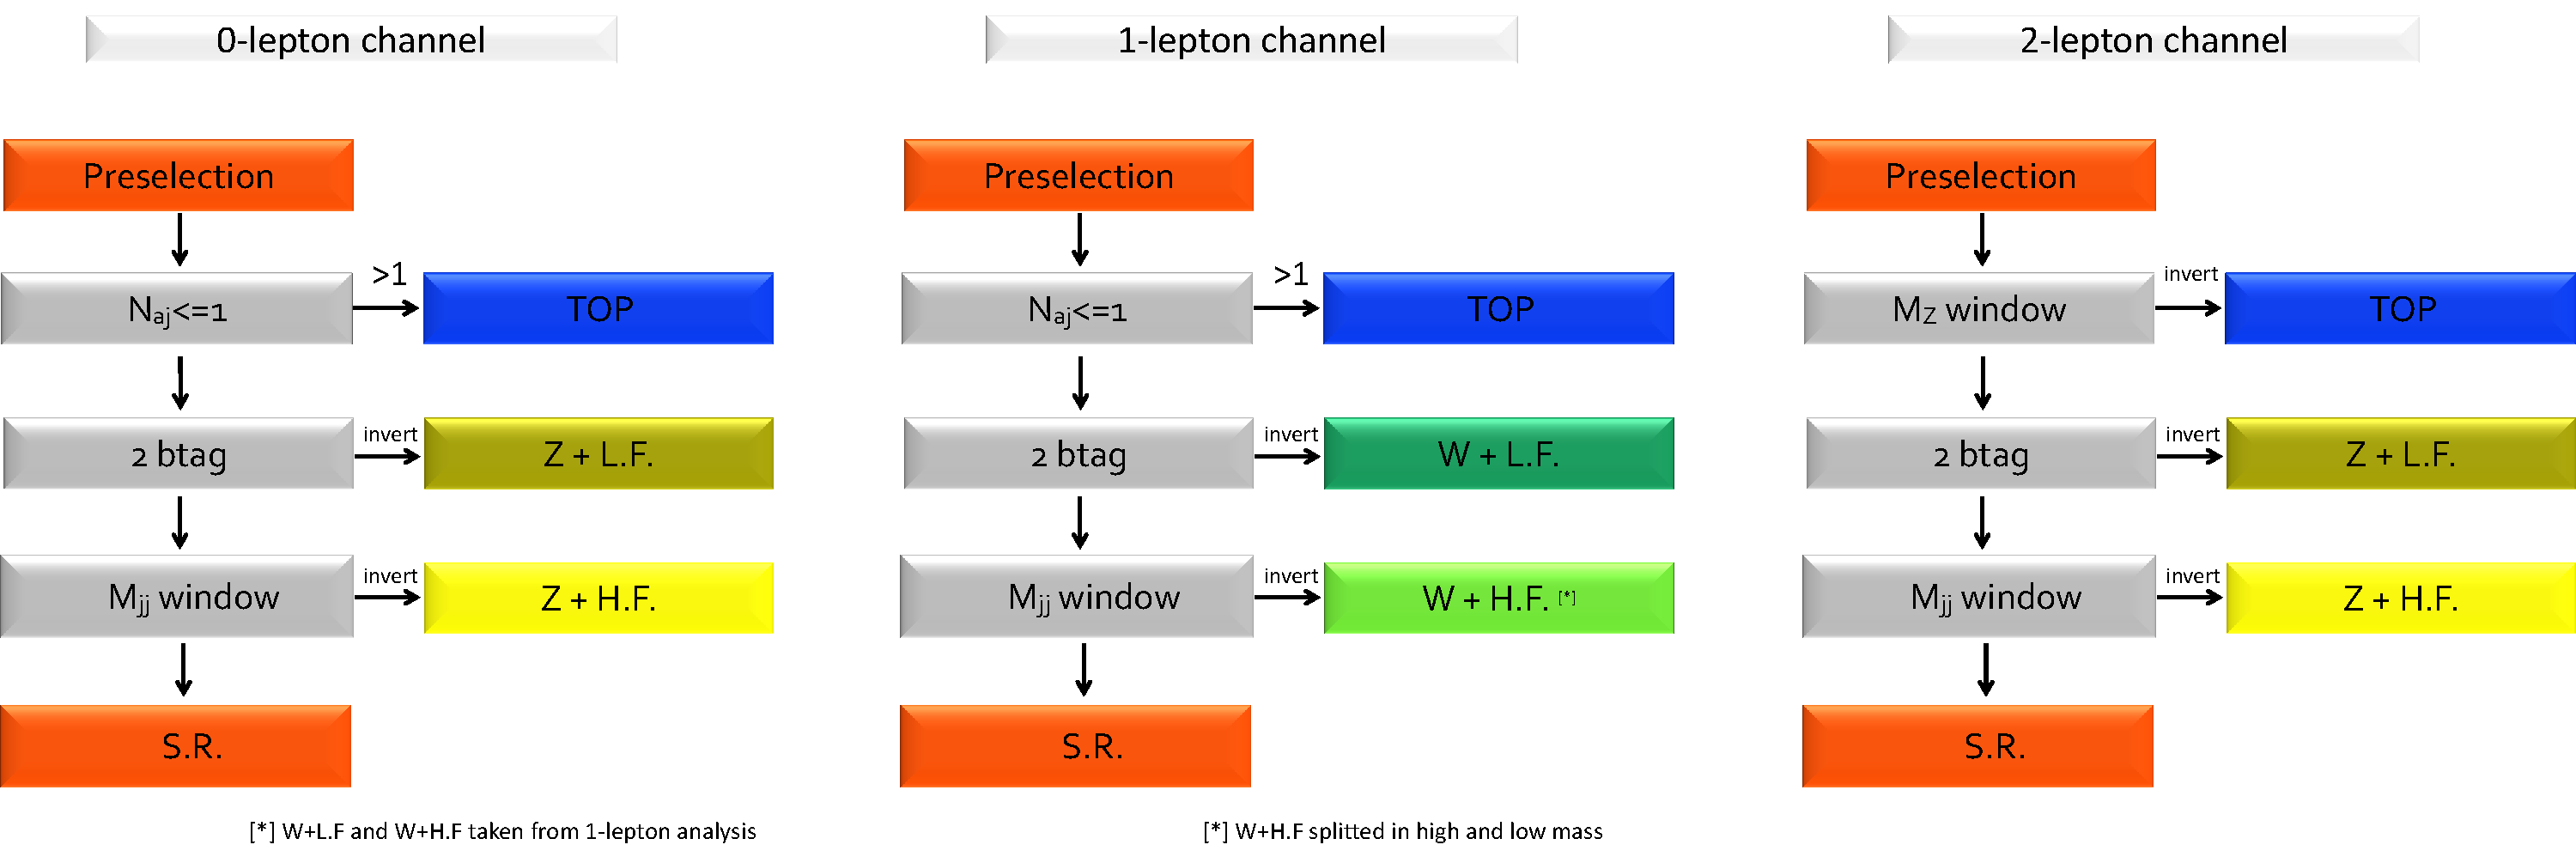
\includegraphics[width=6in]{images/CR_VH}
    \caption[\VHbb\ Control Region Definitions]{An infographic summarizing the inverted cuts used by each decay channel to define their respective control regions.}
    \label{fig:controlregiondef}
\end{figure}

The detailed cuts which define the control regions of the \ZnnH\ channel are listed in Table \ref{tbl:controlregions_Znn}. The \bosZ+heavy process, where \bosZ+jets events produce at least one \qrkb-jet, is the background process most similar to the \ZnnH\ signal. In order to create a \bosZ+heavy enriched control region, the dijet invariant mass window required for the signal region is simply inverted such that the control region focuses on the mass sidebands. Because \qrkt\qrktbar\ is an important background process that is also present in the \bosZ+heavy control region with relatively large contributions, a dedicated control region enriched in the \qrkt\qrktbar\ process is defined by loosening the signal region's Anti-QCD cut threshold to $\pi/2$, loosening the DeepCSV working point to Medium for \btagmax, and requiring at least two additional jets with $\pT > 30\ \GeV$ and at least one additional lepton. The requirement of at least one additional lepton can result in overlap with the \qrkt\qrktbar\ control region for the \WlnH\ channel, so care is taken to ensure that these two control regions remain distinct. A control region enriched in the \bosZ+light process, where \bosZ+jets events produce only light flavored jets, is defined by removing the dijet invariant mass window and inverting the DeepCSV working point cut placed on \btagmax, creating a fairly pure control region that helps to constrain the normalization of the background process.

The detailed cuts which define the control regions of the \WlnH\ and \ZllH\ channels are listed in Table \ref{tbl:controlregions_Wln} and Table \ref{tbl:controlregions_Zll}, respectively.  Distributions of important variables in all of the control regions of the different decay channels are found in Appendix \ref{appendixB}. Because the \bosW+jets processes can have large relative contributions in the \bosZ+light and \bosZ+heavy control regions of the \ZnnH\ channel, the \bosW+light and \bosW+heavy control regions of the \WlnH\ channel are adopted by the \ZnnH\ channel to constrain the normalization of those processes.

\begin{table}[htbp]
  \caption[\ZnnH\ Control Region Definitions for the 2017 \VHbb\ Analysis]{The cuts defining the control regions of the \ZnnH\ decay channel for the \VHbb\ analysis. The values of the kinematic quantities are quoted in \GeV\ and the values of the differences in azimuthal angle are quoted in radians.}
  \label{tbl:controlregions_Znn}
  \begin{tabularx}{6.5in}{XXXX}
    \hline
    Variable                              & \qrkt\qrktbar & \bosZ+light & \bosZ+heavy        \\
    \hline
    \bosV Decay Type                      & \Wmn          & \Znn        & \Znn               \\
    \pTmiss                               & $>170$        & $>170$      & $>170$             \\
    $m(jj)$                               & --            & --          & $\notin [60, 160]$ \\
    $\pT(jj)$                             & $>120$        & $>120$      & $>120$             \\
    \btagmax                              & $>$ Medium    & $<$ Medium  & $>$ Tight          \\
    \btagmin                              & $>$ Loose     & $>$ Loose   & $>$ Loose          \\
    \pTjmax                               & $>60$         & $>60$       & $>60$              \\
    \pTjmin                               & $>35$         & $>35$       & $>35$              \\
    $| \Delta\phi(\bosV, \bosH) |$        & $>2.0$        & $>2.0$      & $>2.0$             \\
    $N_{\mathrm{\ell}}^{\mathrm{add}}$    & $\geq1$       & $=0$        & $=0$               \\
    $N_{\mathrm{j}}^{\mathrm{add}}$       & $\geq2$       & $\leq1$     & $\leq1$            \\
    $| \Delta\phi(\pTmiss, \pTmisstrk) |$ & --            & $<0.5$      & $<0.5$             \\
    $\mathrm{Anti\text{-}QCD}$            & Modified      & Yes         & Yes                \\
    \hline
  \end{tabularx}
\end{table}

\begin{table}[htbp]
  \caption[\WlnH\ Control Region Definitions for the 2017 \VHbb\ Analysis]{The cuts defining the control regions of the \WenH\ and \WmnH\ decay channels for the \VHbb\ analysis. The values of the kinematic quantities are quoted in \GeV\ and the values of the differences in azimuthal angle are quoted in radians. The $\pTmiss \mathrm{Significance}$ is defined as the ratio of \pTmiss\ to the scalar sum of the transverse energy of all particle-flow objects in the event.}
  \label{tbl:controlregions_Wln}
  \begin{tabularx}{6.5in}{XXXX}
    \hline
    Variable                              & \qrkt\qrktbar & \bosW+light & \bosW+heavy        \\
    \hline
    \bosV Decay Type                      & \Wmn          & \Wmn        & \Wmn               \\
    $\pT(\bosV)$                          & $>150$        & $>150$      & $>150$             \\
    $| \Delta\phi(\pTmiss, \ell) |$       & $<2.0$        & $<2.0$      & $<2.0$             \\
    $m(jj)$                               & $<250$        & $<250$      & $\notin [90, 150]$ \\
    $\pT(jj)$                             & $>100$        & $>100$      & $>100$             \\
    \btagmax                              & $>$ Tight     & $<$ Medium  & $>$ Tight          \\
    \btagmin                              & $>$ Loose     & $>$ Loose   & $>$ Loose          \\
    \pTjmax                               & $>25$         & $>25$       & $>25$              \\
    \pTjmin                               & $>25$         & $>25$       & $>25$              \\
    $| \Delta\phi(\bosV, \bosH) |$        & $>2.5$        & $>2.5$      & $>2.5$             \\
    $N_{\mathrm{\ell}}^{\mathrm{add}}$    & $\geq1$       & --          & $=0$               \\
    $N_{\mathrm{j}}^{\mathrm{add}}$       & --            & $\geq1$     & $\leq1$            \\
    $| \Delta\phi(\pTmiss, \pTmisstrk) |$ & --            & $<0.5$      & $<0.5$             \\
    $\pTmiss \mathrm{Significance}$       & --            & $>2.0$      & $>2.0$             \\
    \hline
  \end{tabularx}
\end{table}

\begin{table}[htbp]
  \caption[\ZllH\ Control Region Definitions for the 2017 \VHbb\ Analysis]{The cuts defining the control regions of the \ZeeH\ and \ZmmH\ decay channels for the \VHbb\ analysis. The values of the kinematic quantities are quoted in \GeV\ and the values of the differences in azimuthal angle are quoted in radians.}
  \label{tbl:controlregions_Zll}
  \begin{tabularx}{6.5in}{XXXX}
    \hline
    Variable                              & \qrkt\qrktbar                      & \bosZ+light       & \bosZ+heavy        \\
    \hline
    \bosV Decay Type                      & \Zll                               & \Zll              & \Zll               \\
    $\pT(\bosV)$                          & $[50, 150], >150$                  & $[50, 150], >150$ & $[50, 150], >150$  \\
    $m(\ell\ell)$                         & $\notin [0, 10], \notin [75, 120]$ & $[75, 105]$       & $[85, 97]$         \\
    $m(jj)$                               & --                                 & $[90, 150]$       & $\notin [90, 150]$ \\
    \btagmax                              & $>$ Tight                          & $<$ Loose         & $>$ Tight          \\
    \btagmin                              & $>$ Loose                          & $<$ Loose         & $>$ Loose          \\
    \pTjmax                               & $>20$                              & $>20$             & $>20$              \\
    \pTjmin                               & $>20$                              & $>20$             & $>20$              \\
    $| \Delta\phi(\bosV, \bosH) |$        & --                                 & $>2.5$            & $>2.5$             \\
    \pTmiss                               & --                                 & --                & $<60$              \\
    \hline
  \end{tabularx}
\end{table}

\section{Binned Multivariate Shape Analysis}

In order to observe the \VHbb\ decay, the distributions considered by the signal extraction fit must enable the hypothesized \VHbb\ signal to be distinguished from the SM background. Although the dijet invariant mass distribution is a powerful physical observable on its own, statistical learning methods can leverage the information spread across multiple key variables to further separate the signal from background. Because multivariate discriminants can achieve signal-to-background ratios which exceed those of individual physical observables, a multivariate approach is employed by this analysis to maximize the sensitivity to the signal process.

\subsection{Multivariate Discriminator}

For this analysis, the multivariate discriminator is a classifier with a single, continuous valued output that scores events based on how ``signal-like'' they appear, with the convention that more ``signal-like'' events receive higher scores. Because the final state topologies and background contributions are specific to each decay channel, separate instances of the classifier are trained for the \ZnnH, \WlnH, and the low and high $\pT(\bosV)$ \ZllH\ categories, where the training may be inclusive or exclusive for the \lepe\ and \lepm\ final states. The discriminant distributions of these distinct models are used for the final signal extraction.

The classifiers are trained in a supervised manner using the MC simulated events which pass the signal region selection of their respective decay channel. For each decay channel, the simulated events are further divided into a training set and a validation set based on the parity of their generator level ID values to obtain two statistically independent samples which are roughly equal in size, typically around 200,000 events. The training set is used solely to train the classifier while the validation set is used to evaluate the generalization performance of the model and tune the hyperparameters of the machine learning algorithm. Because of the limited statistics available for the 2017 MC samples, the classifiers are trained and validated using the 2016 MC samples while the 2017 MC samples are used to provide the signal region discriminant distribution considered by the signal extraction fit.

The variables which are used as the classifier input features are listed in Table \ref{tbl:inputfeatures}. The final set of input features were selected using a ``leave-one-out'' strategy, where an initial subset of variables chosen based on their physics efficacy for each channel are further refined by iteratively holding out one variable while training the classifier with the rest. By evaluating the performance of each of these classifiers on the validation set, an optimal set of input features is determined. Because the training and validation sets are derived from 2016 MC samples but the 2017 MC samples and data are used for the signal extraction fit, a lack of agreement between the data and simulated samples in the distributions of the input variables could jeopardize the generalizability of the classifier. It is found that the distributions of the input features remain fairly consistent between the 2016 and 2017 MC samples. 

\begin{table}[htbp]
  \caption[Event Classification Variables]{The variables which define the input features used to train the event classifier models for the multivariate discriminant analysis. The values of the kinematic quantities are quoted in \GeV\ and the values of the differences in azimuthal angle are quoted in radians.}
  \label{tbl:inputfeatures}
  \small
  \begin{tabularx}{6.5in}{lXrrr}
    \hline
    Variable                        & Description                                                                               & \ZnnH      & \WlnH      & \ZllH      \\
    \hline
    $m(jj)$                         & dijet invariant mass                                                                      & \checkmark & \checkmark & \checkmark \\
    $\pT(jj)$                       & dijet transverse momentum                                                                 & \checkmark & \checkmark & \checkmark \\
    \pTjmax, \pTjmin                & transverse momentum of the two \qrkb-jets                                                 & \checkmark &            & \checkmark \\
    $\Delta R(jj)$                  & distance between the two \qrkb-jets in $\eta$-$\phi$ space                                &            &            & \checkmark \\
    $\Delta \eta(jj)$               & difference in $\eta$ between the two \qrkb-jets                                           & \checkmark &            & \checkmark \\
    $\Delta \phi(jj)$               & difference in $\phi$ between the two \qrkb-jets                                           & \checkmark &            &            \\
    $\pT(\bosV)$                    & vector boson transverse momentum                                                          &            & \checkmark & \checkmark \\
    $\Delta \phi(\bosV, \bosH)$     & difference in $\phi$ between the dijet system and vector boson                            & \checkmark & \checkmark & \checkmark \\
    $\pT(jj) / \pT(\bosV)$          & \pT\ ratio of the dijet system to the vector boson                                        &            &            & \checkmark \\
    $m(\bosZ)$                      & reconstructed mass of the \bosZ\ boson                                                    &            &            & \checkmark \\
    \btagmax                        & leading DeepCSV score of the two \qrkb-jets                                               & \checkmark &            & \checkmark \\
    \btagmin                        & subleading DeepCSV score of the two \qrkb-jets                                            & \checkmark & \checkmark & \checkmark \\
    \btagadd                        & leading DeepCSV score of all additional jets                                              & \checkmark &            &            \\
    \pTmiss                         & missing transverse energy                                                                 & \checkmark & \checkmark & \checkmark \\
    $|\Delta\phi(\pTmiss, j)|$      & difference in $\phi$ between \pTmiss\ and the nearest jet with $\pT > 30\ \GeV$           & \checkmark &            &            \\
    $|\Delta\phi(\pTmiss, \ell)|$   & difference in $\phi$ between \pTmiss\ and the isolated lepton                             &            & \checkmark &            \\
    $m_{\mathrm{T}}$                & mass of the isolated lepton $\vec{p}_{\mathrm{T}} + \vec{p}_{\mathrm{T}}^{\mathrm{miss}}$ &            & \checkmark &            \\
    $m_{\qrkt}$                     & reconstructed mass of the top quark                                                       &            & \checkmark &            \\
    $N_{\mathrm{j}}^{\mathrm{add}}$ & number of additional jets                                                                 &            & \checkmark & \checkmark \\
    \pTjadd                         & highest \pT\ of all additional jets                                                       & \checkmark &            &            \\
    SA5                             & number of soft-track jets with $\pT > 5\ \GeV$                                            & \checkmark & \checkmark & \checkmark \\
    \hline
  \end{tabularx}
\end{table}

\begin{figure}[htbp]
  \centering
    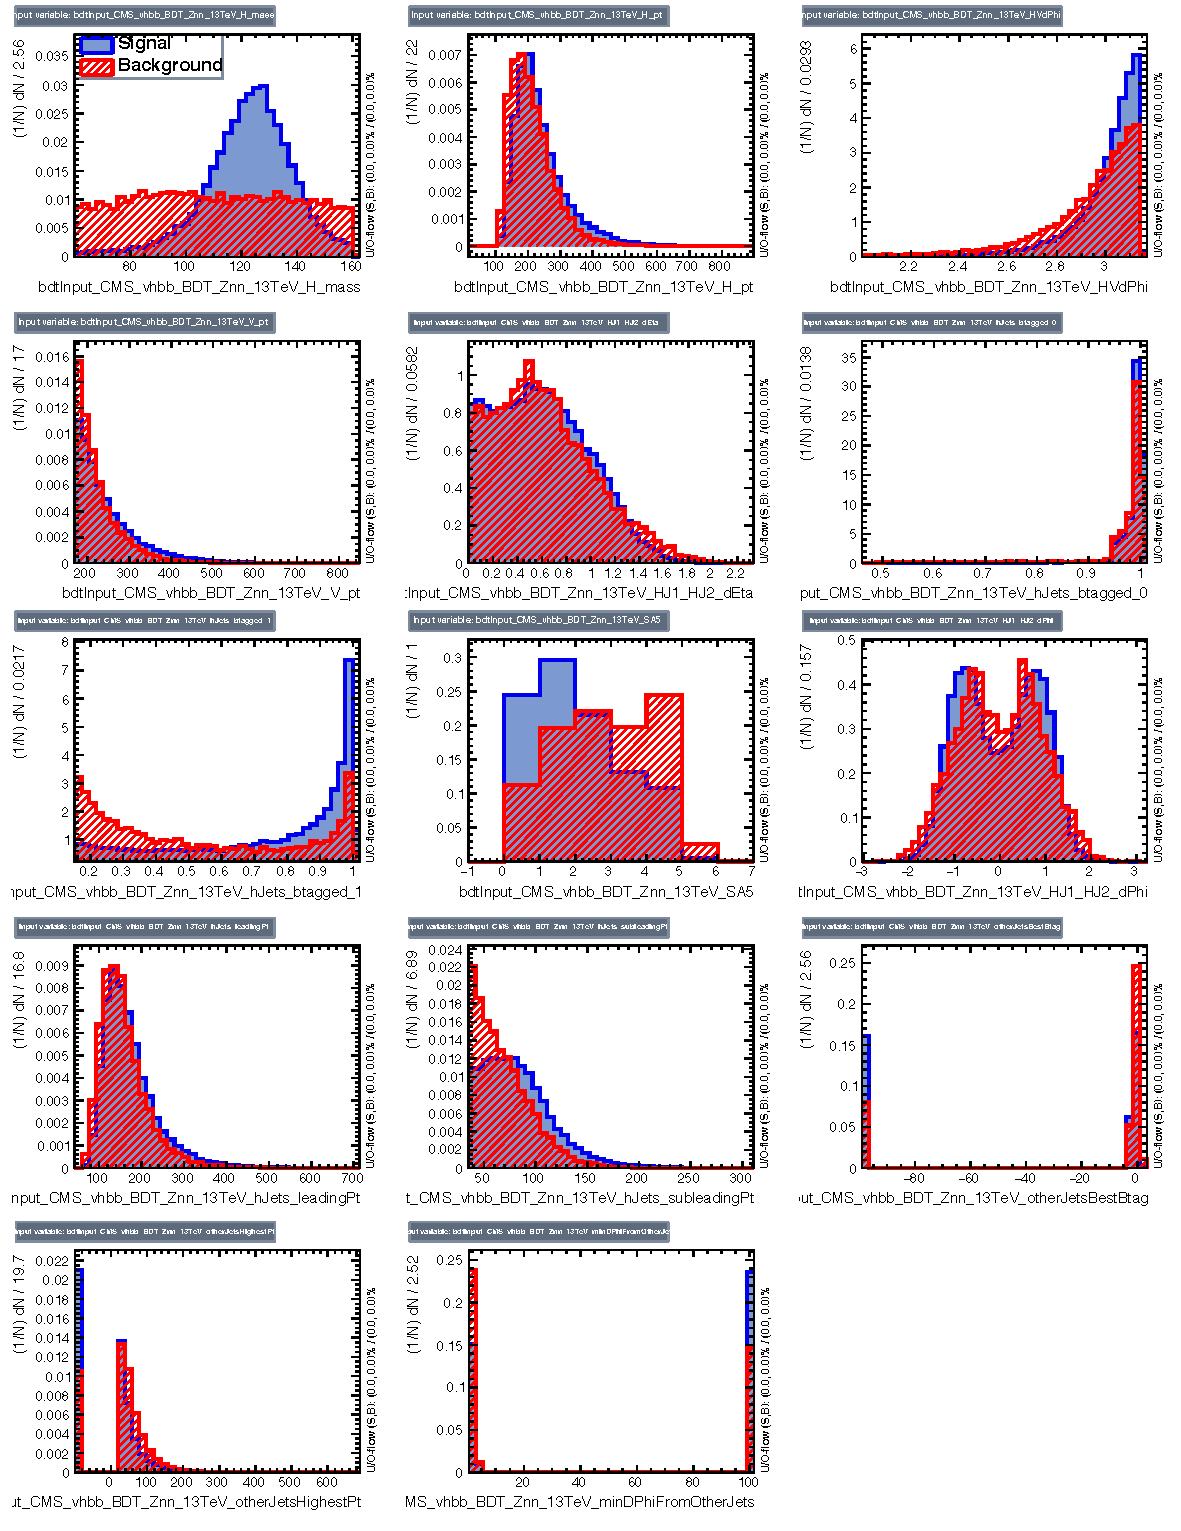
\includegraphics[width=6in]{images/features_Znn}
    \caption[Input Feature Distributions for the \ZnnH\ Channel]{The distributions of select input features for the \ZnnH\ decay channel. In order to emphasize the separation between signal (blue) and background (red), the distributions are normalized.}
    \label{fig:features_Znn}
\end{figure}

Two different machine learning algorithms were considered for the final multivariate discriminant. Gradient boosted decision tree (BDT)\cite{GBDT} classifiers implemented using the \texttt{TMVA} v4.2.1\cite{TMVA} software package were used to establish a performance baseline, given their broad acceptance by the high energy physics community because of the relative interpretability of their results and good ``out-of-the-box'' performance with little to no input feature preprocessing or hyperparameter tuning. Multilayer perceptron\cite{MLP} or artificial neural network (ANN) classifiers implemented using the \texttt{Keras} neural network framework with \texttt{Tensorflow} as the computational backend were compared to the incumbent BDT classifiers to determine if recent advances in the implementation and training of ANN classifiers resulted in superior performance.

Optimal BDT and ANN classification models were selected using a grid-based hyperparameter search with the area under the receiver operating characteristic (ROC) curve evaluated on the validation set as the performance metric. Because overfitting can result in models which fail to generalize because they are sensitive to fine variations in the training set, the Kolmogorov-Smirnov test statistic was used to estimate the compatibility of the discriminant distribution of the training set to the validation set. The compatibility of the normalized shapes of the discriminant distributions for the training and validations sets were also visually inspected.

The performance of the optimized BDT and ANN classifiers were found to be nearly equivalent, with both models achieving similar area under the ROC curve values near 0.80 when evaluated on the validation set. The ANN classifier was chosen as the final discriminantor for the analysis. The chosen neural network architecture, dubbed ``DNN'' for deep neural network, takes as input the training features of a specific decay channel, each scaled to zero mean and unit variance, and passes them through five hidden layers with 32 nodes in each layer. The hidden layer nodes are Leaky ReLU units with a slope of $\beta = 0.2$ for the negative part of its argument. Residual connections\cite{RESCONNECT}, which have been shown to benefit the training of deep neural networks by mitigating the problem of vanishing or exploding gradients during training, were made between the first, second, and third hidden layers and the last hidden layer and between the second and fourth hidden layers. Batch-normalization and dropout with a probability of 0.1 are applied to the outputs of each hidden layer to increase the training speed and regularize the model. The output layer consists of two linear nodes passed through a softmax activation function. A softmax output layer was chosen because the output values are interpreted to be the probability that an event belongs to one of the two possible classes of signal or background. The DNN was trained to minimize the cross entropy loss using stochastic gradient descent with adaptive moment estimation, or the Adam optimizer. The output node of the DNN chosen to represent the probability that an event belongs to the signal class defines a discriminant whose values fall within the inclusive range $[0, 1]$, where events with lower scores are more background-like and events with higher scores are more signal-like. The normalized discriminant distributions of each of the trained DNN classifiers are shown in Figure \ref{fig:DNN_overtrain}. 

\begin{figure}[htbp]
  \centering
  \mbox{
    \subfigure [] {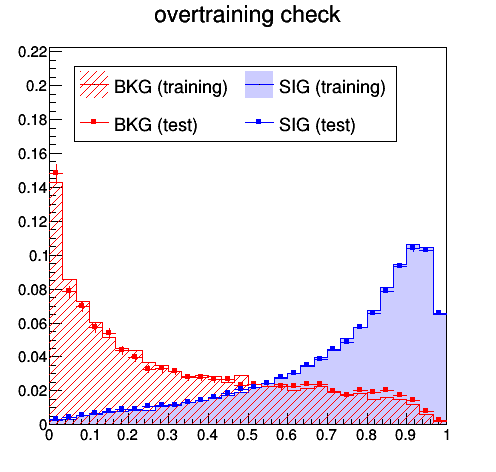
\includegraphics[width=0.38\linewidth]{images/Zll_low_overtraining}}
    \subfigure [] {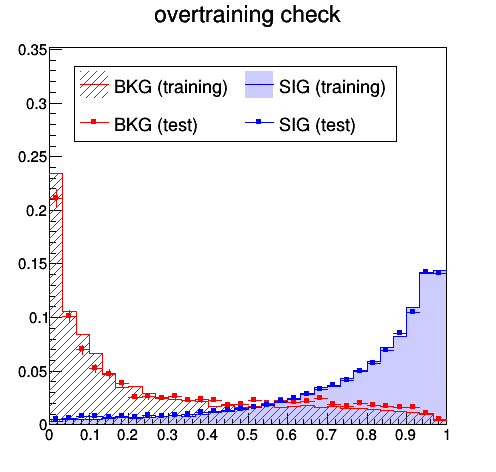
\includegraphics[width=0.38\linewidth]{images/Zll_high_overtraining}}
  }
  \mbox{
    \subfigure [] {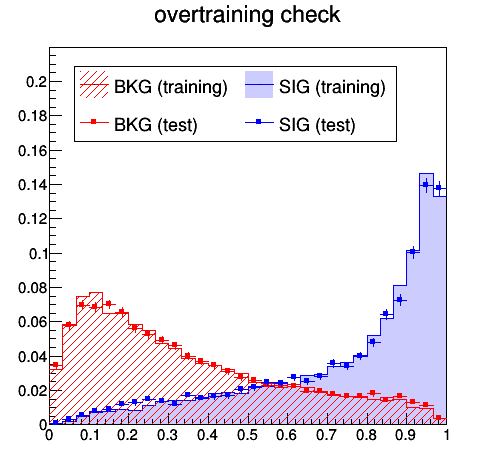
\includegraphics[width=0.38\linewidth]{images/Wen_overtraining}}
    \subfigure [] {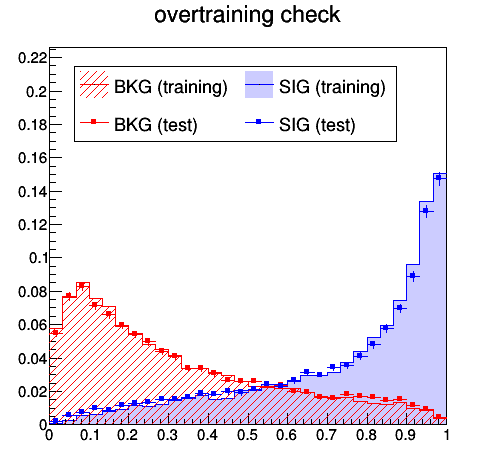
\includegraphics[width=0.38\linewidth]{images/Wmn_overtraining}}
  }
  \mbox{
    \subfigure [] {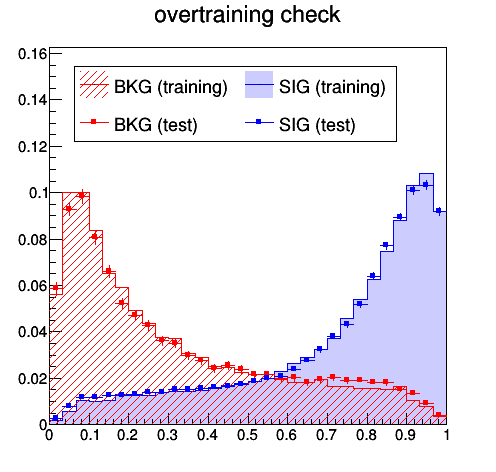
\includegraphics[width=0.38\linewidth]{images/Znn_overtraining}}
  }
  \caption[Normalized DNN Discriminant Distributions]{The normalized DNN discriminant distributions for the A) low $\pT(\bosV)$ \ZllH; B) high $\pT(\bosV)$ \ZllH; C) \WenH; D) \WmnH; and E) \ZnnH\ channels. The signal distributions are shown for the training set (solid blue) and for the validation set (blue points). The background distributions are also shown for the training set (hashed red) and the validation set (red points).}
  \label{fig:DNN_overtrain}
\end{figure}

Because the \bosZ+heavy control region of the \ZnnH\ channel and the \bosW+heavy control region of the \WlnH\ channel are not pure in the enriched background, the normalization of the \bosV+\qrkb\ and \bosV+\qrkb\qrkbbar\ processes are difficult to constrain. A variation of the DNN is therefore used to enhance the separation of the contributing background processes in the \bosV+heavy flavor control regions of the \ZnnH\ and \WlnH\ channels. The input features are the same as those used for the signal classification task, except that the training and validation events pass the control region selection of their respective decay channel. The training is carried out as before, with the neural network architecture modified to use a five-way softmax output layer whose values are interpreted to be the probability that an event belongs to one of five possible background classes: \bosV+\qrkb\qrkbbar, \qrkt\qrktbar, \bosV+light, \bosV+\qrkb, and single top. The discriminant distributions of these multi-background DNN classifiers are shown in Figure \ref{fig:DNN_multi}.

\begin{figure}[htbp]
  \centering
  \mbox{
    \subfigure [] {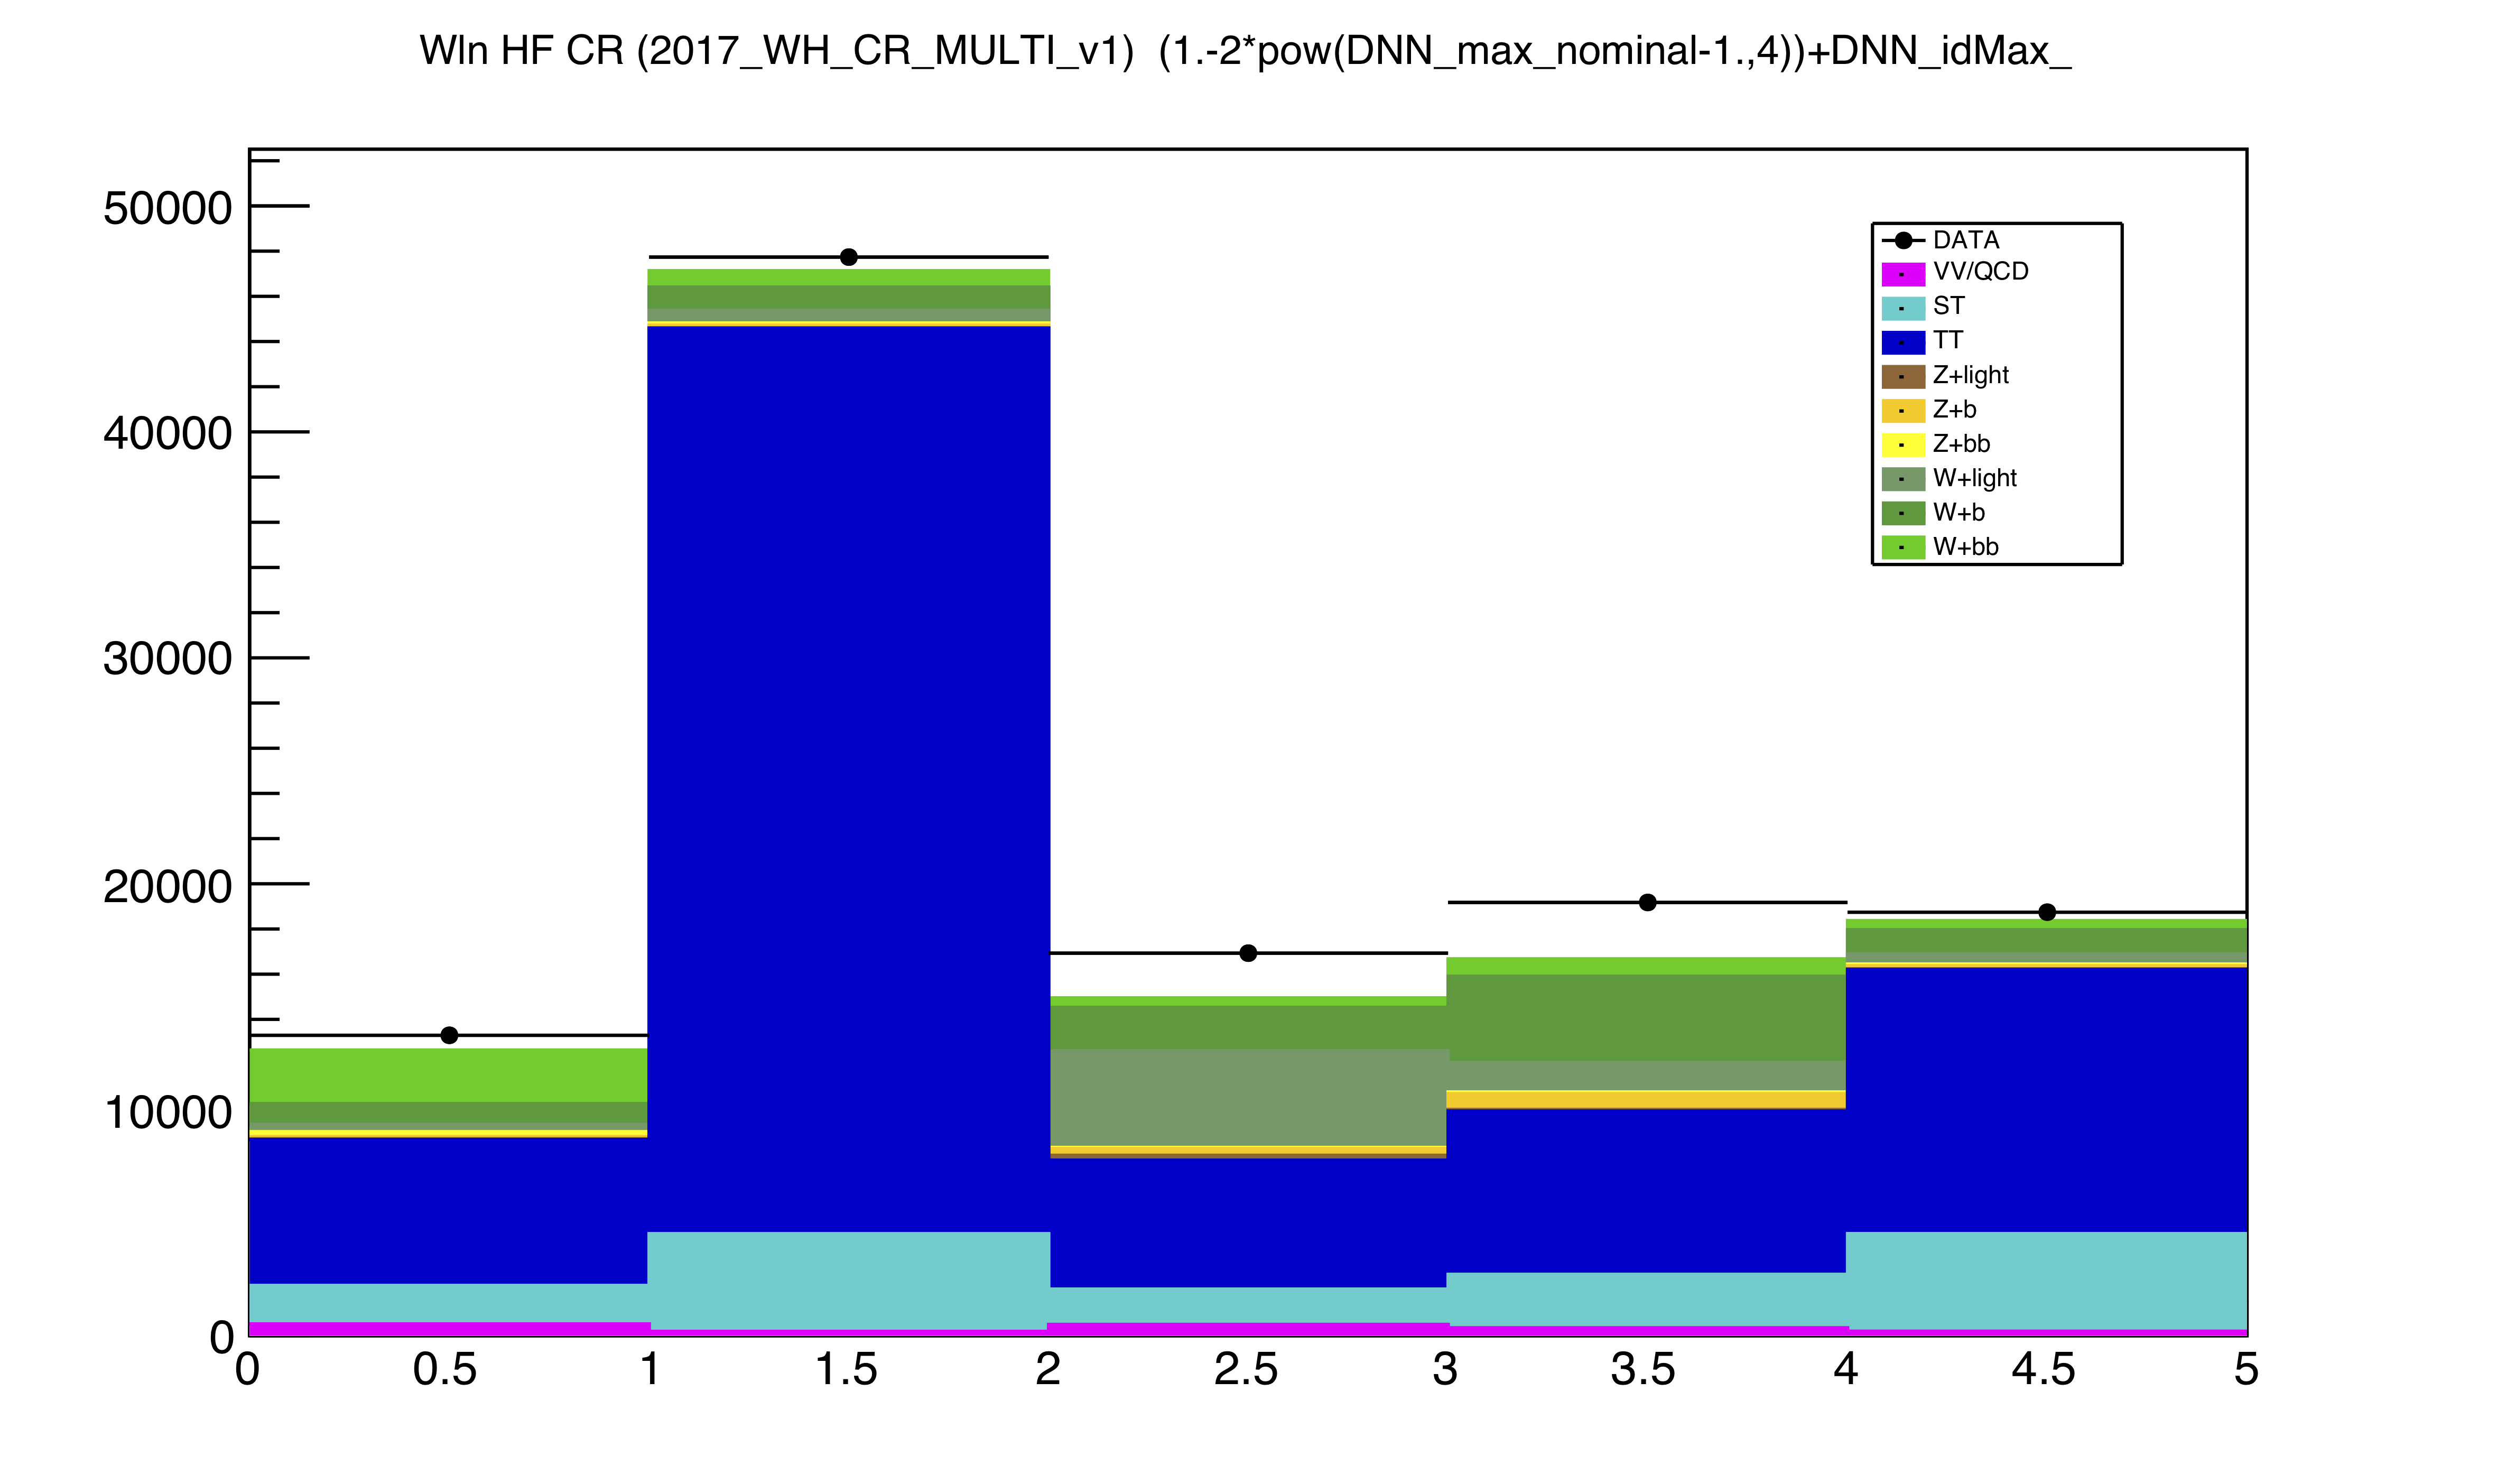
\includegraphics[width=0.38\linewidth]{images/AT_2017_WH_CR_MULTI_v1_5bins}}
    \subfigure [] {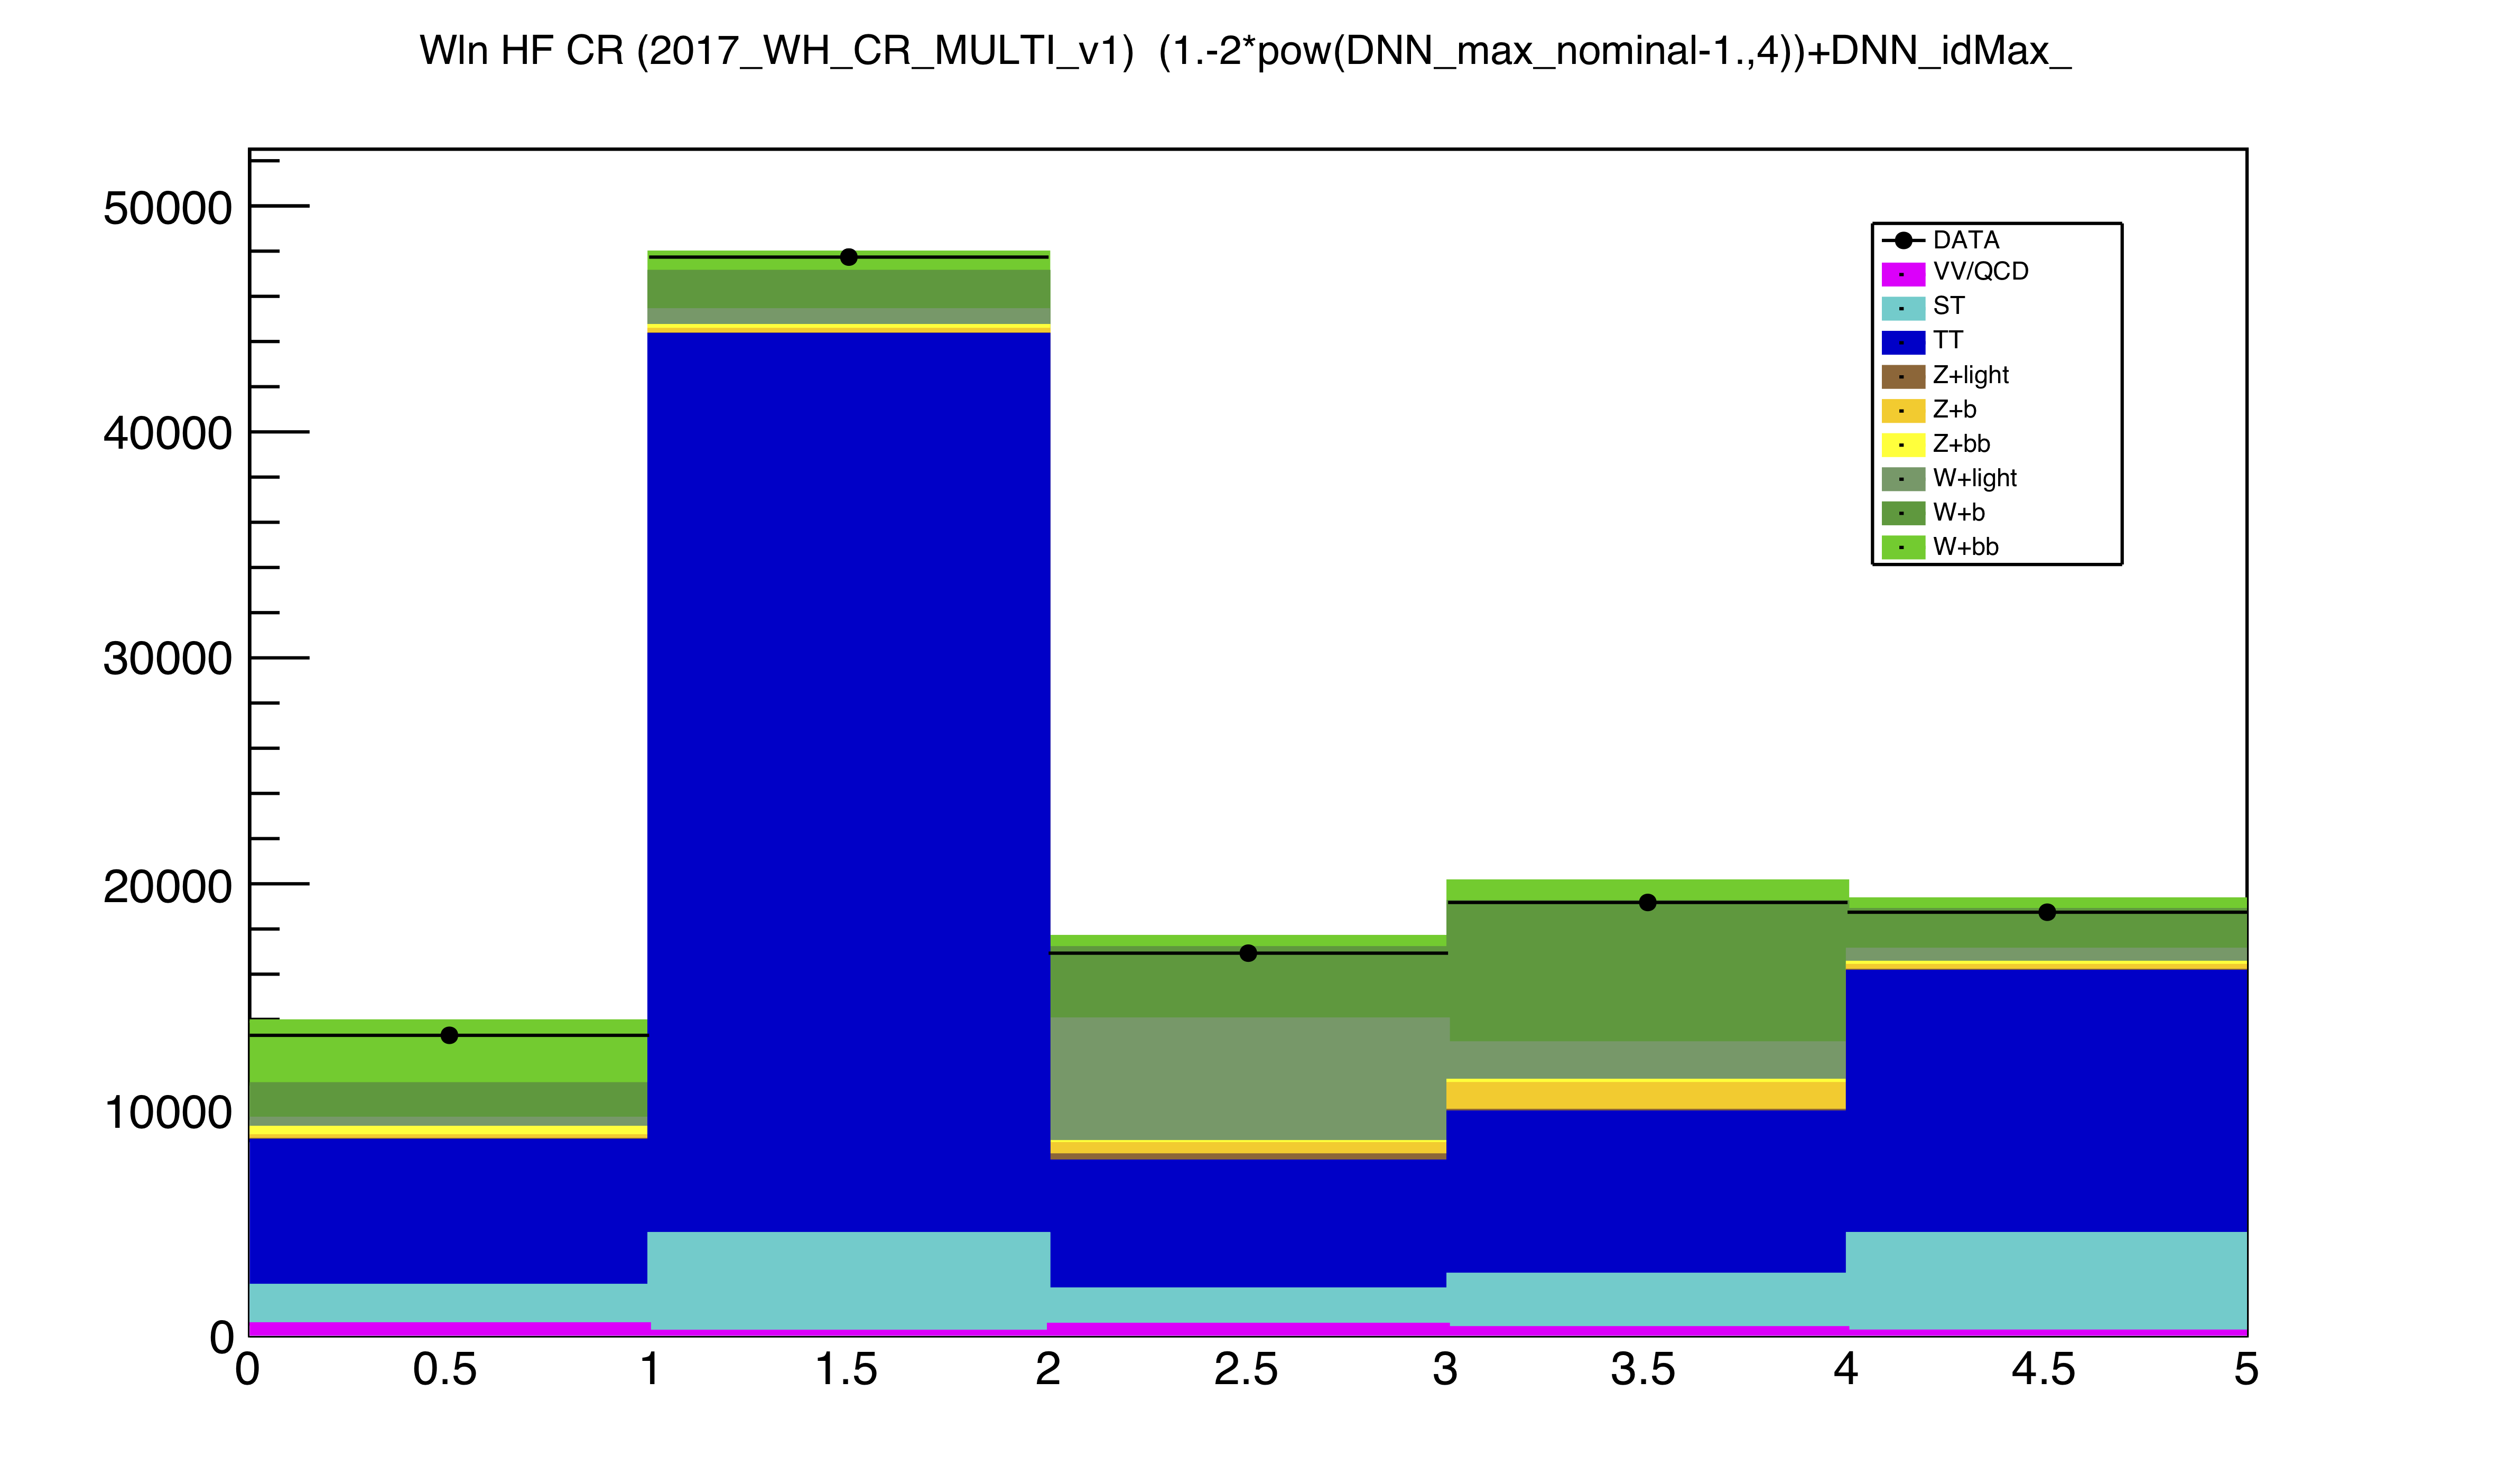
\includegraphics[width=0.38\linewidth]{images/AT_2017_WH_CR_MULTI_v1_5bins_SF}}
  }
  \mbox{
    \subfigure [] {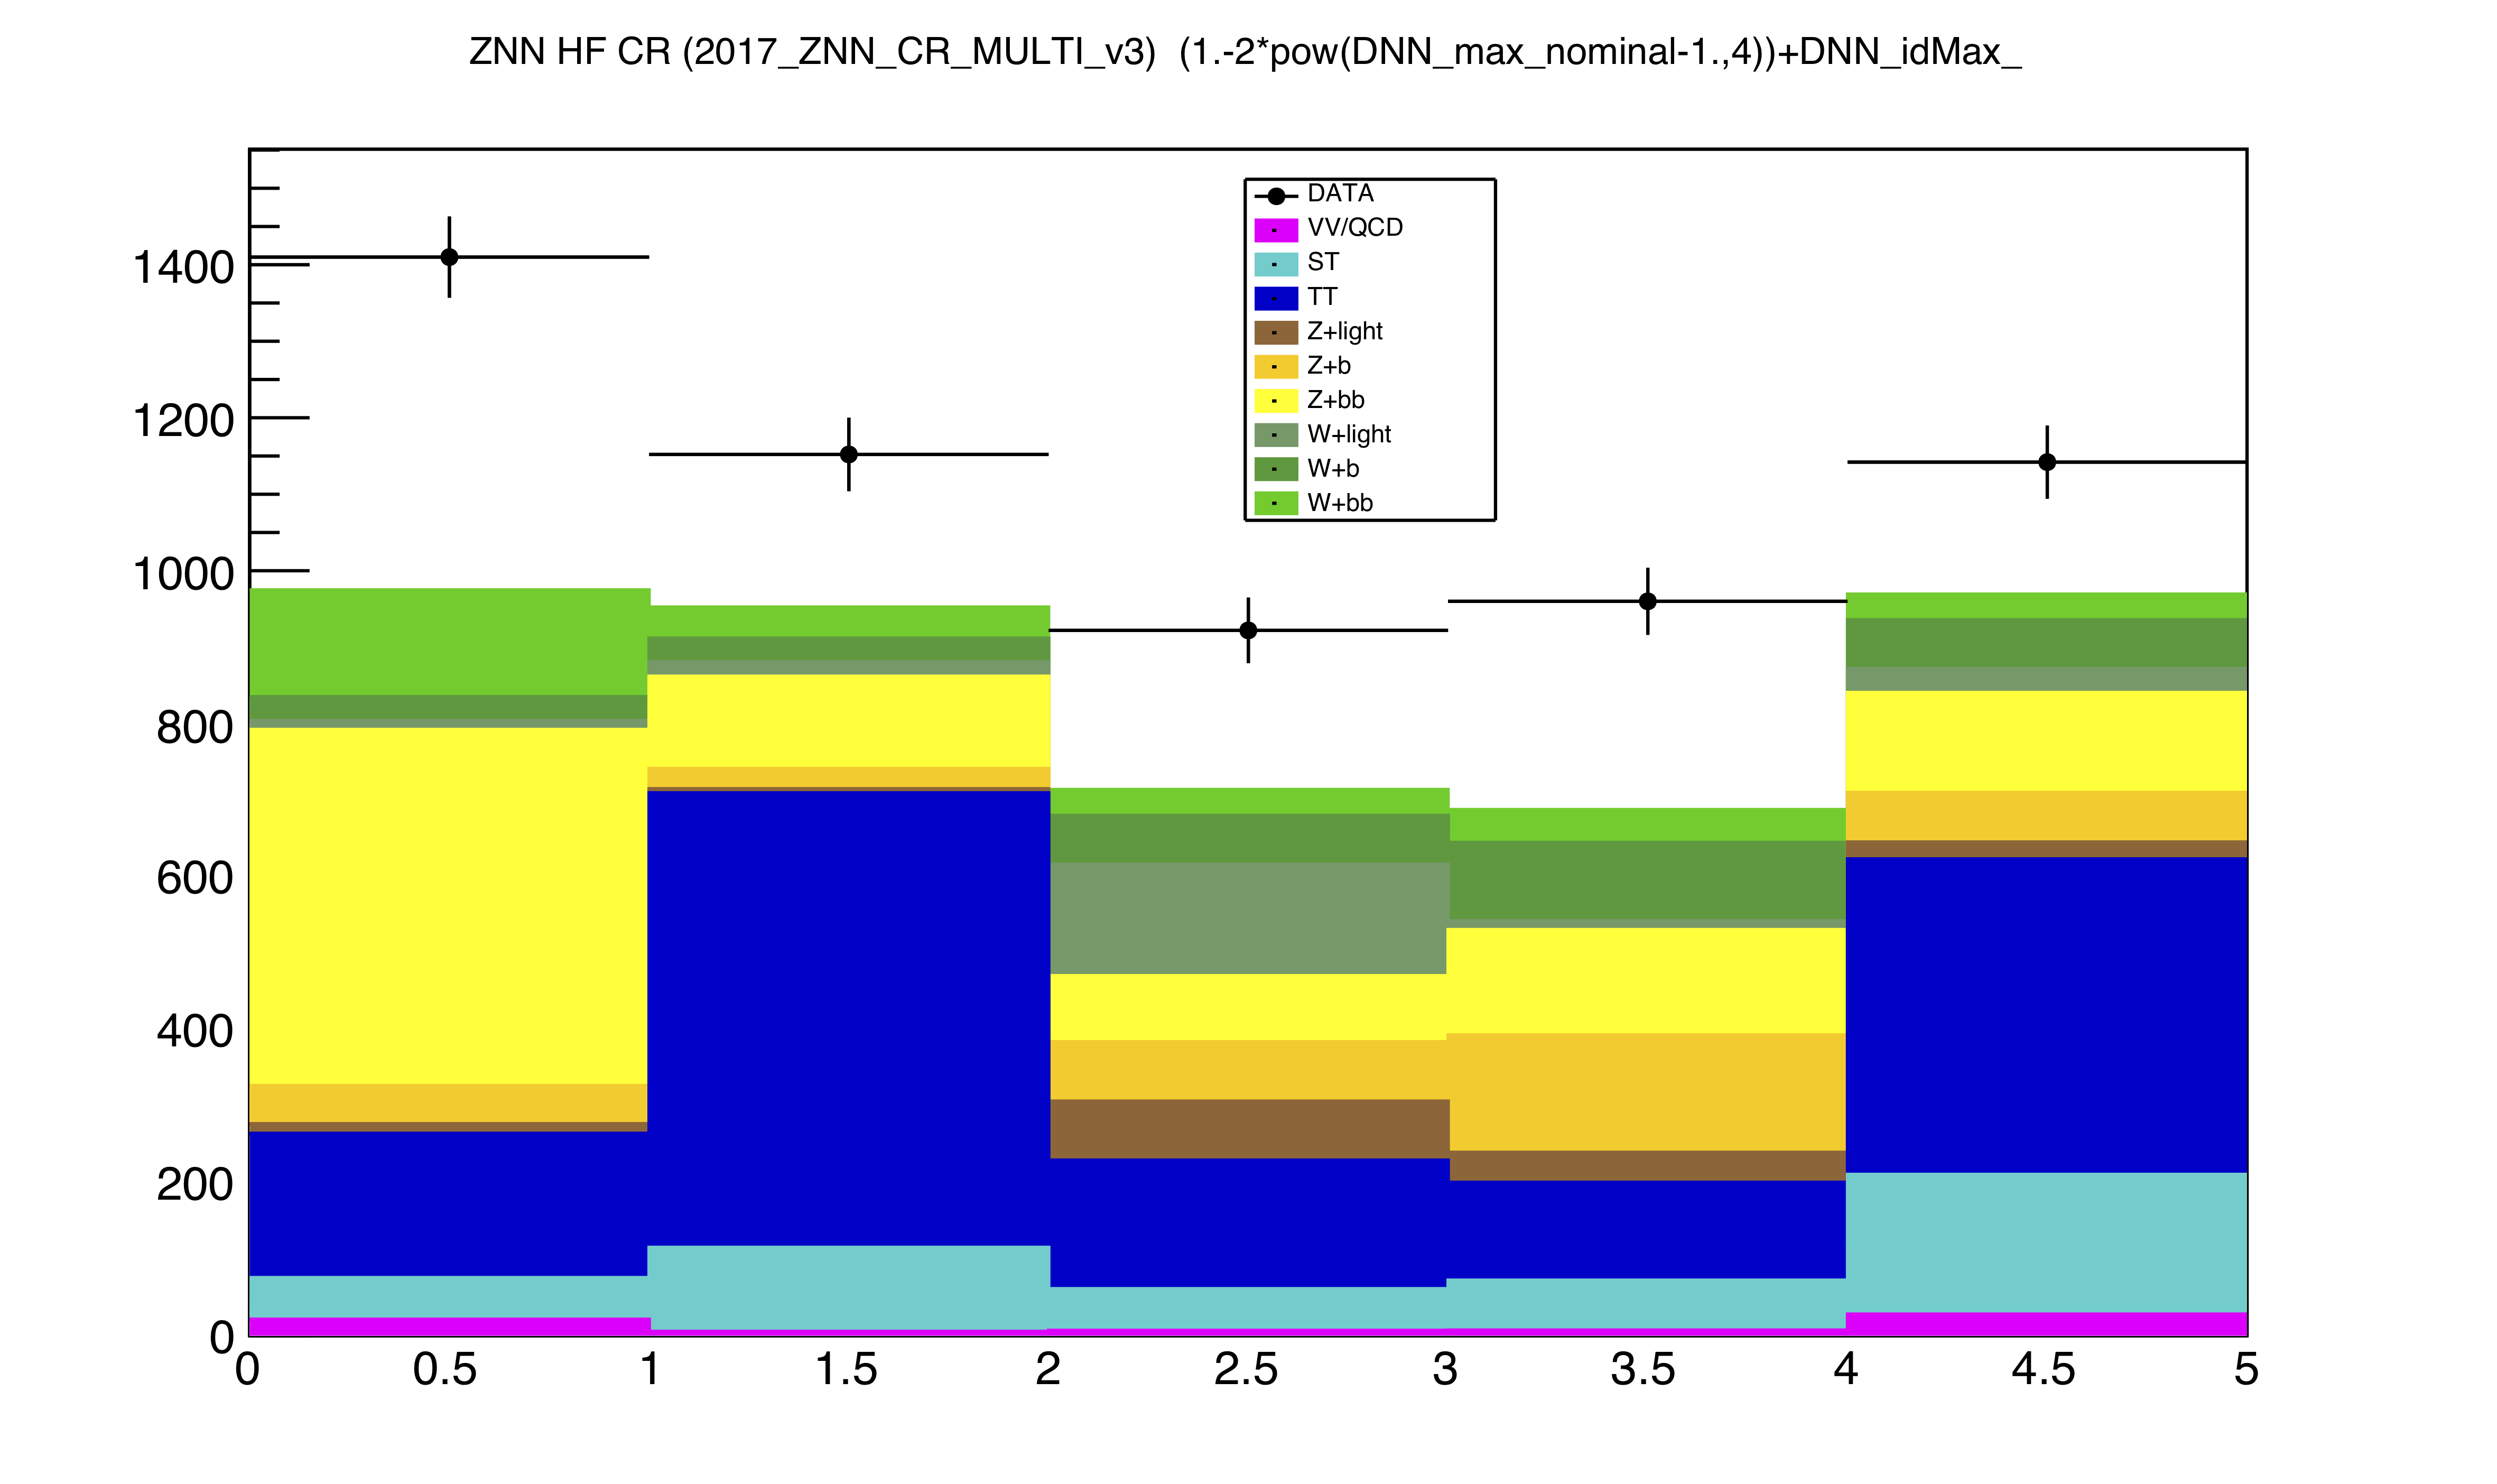
\includegraphics[width=0.38\linewidth]{images/AT_2017_ZNN_CR_MULTI_v3_5bins}}
    \subfigure [] {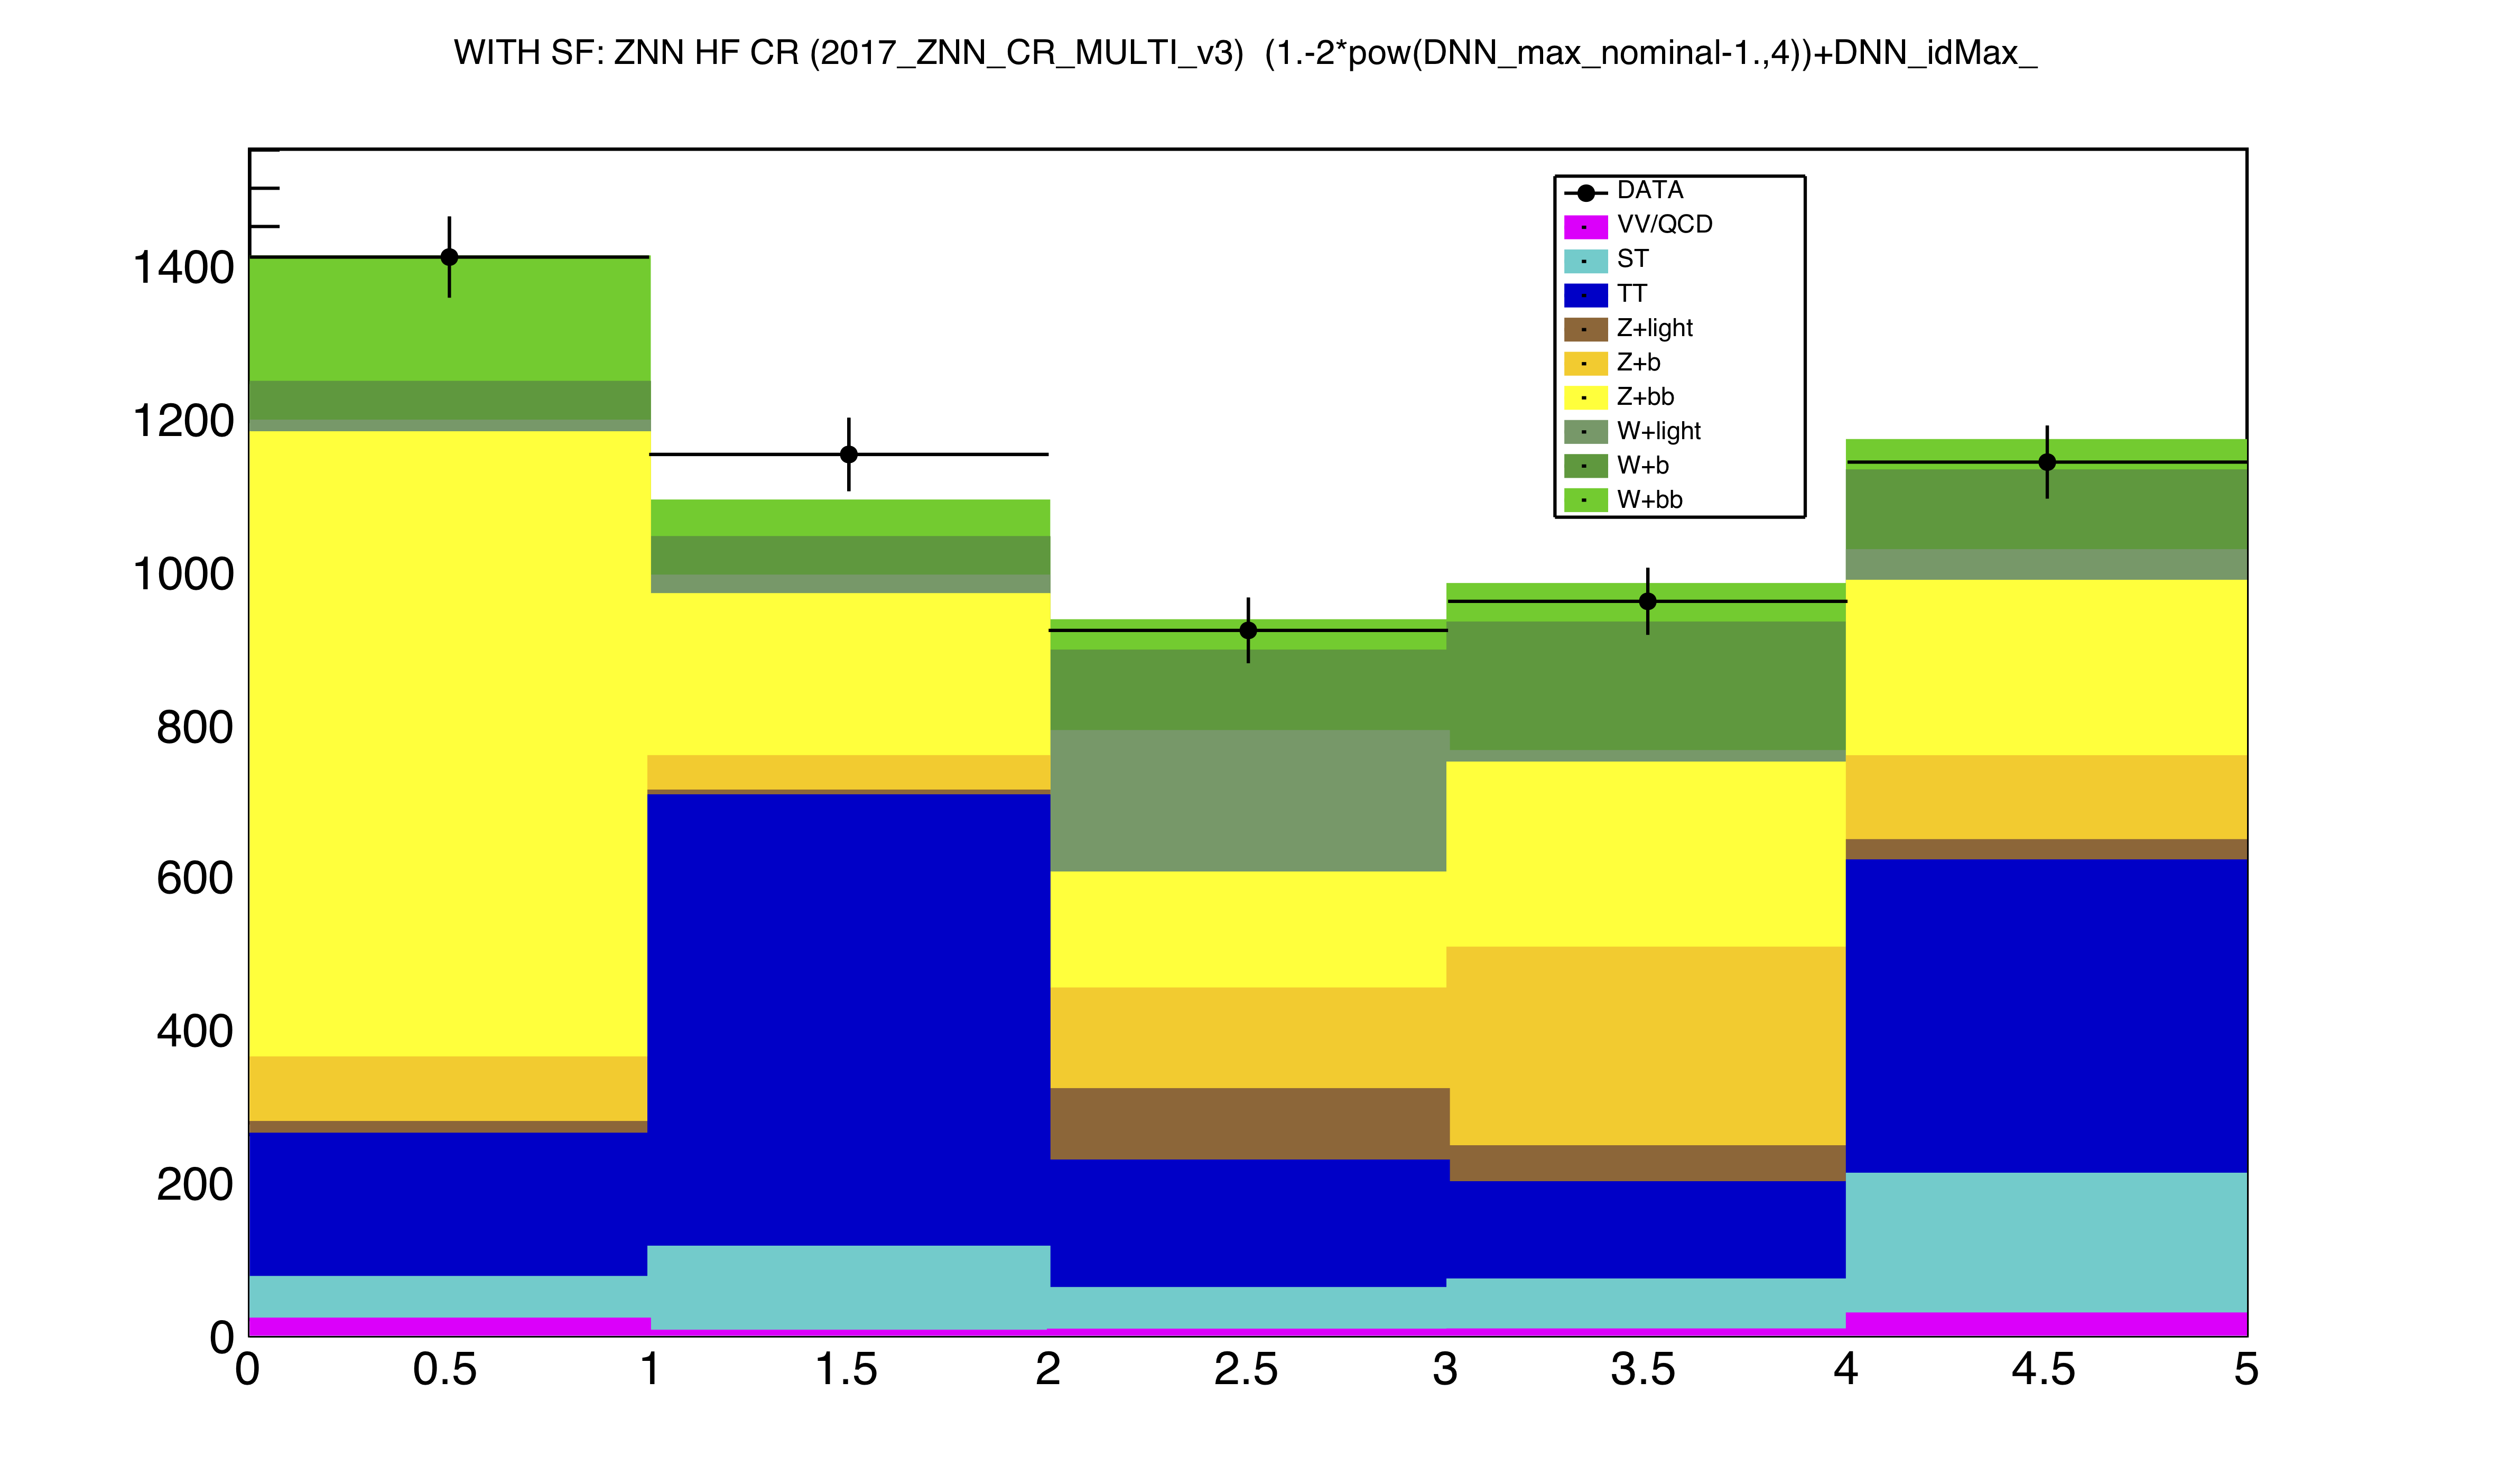
\includegraphics[width=0.38\linewidth]{images/AT_2017_ZNN_CR_MULTI_v3_5bins_SF}}
  }
  \caption[Multi-background DNN Discriminant Distributions]{The multi-background DNN discriminant distributions for the \bosW+heavy control region of the \WlnH\ channel (top row) and \bosZ+heavy control region of the \ZnnH\ channel (bottom row) both A), C) before and B), D) after the background process normalizations have been adjusted.}
  \label{fig:DNN_multi}
\end{figure}

\subsection{Binned Shape Analysis}

\subsection{Cross-check Analysis}

\subsection{Invariant Mass Analysis}

\section{Systematic Uncertainties}

%\section{Non Porttitor Tellus}
%
%Aliquam molestie sed urna quis convallis. Aenean nibh eros, aliquam non eros in, tempus lacinia justo. In magna sapien, blandit a faucibus ac, scelerisque nec purus. Praesent fermentum felis nec massa interdum, vel dapibus mi luctus. Cras id fringilla mauris. Ut molestie eros mi, ut hendrerit nulla tempor et. Pellentesque tortor quam, mattis a scelerisque nec, euismod et odio. Mauris rhoncus metus sit amet risus mattis, eu mattis sem interdum.
%
%\subsection{Nam Arcu Magna}
%Semper vel lorem eu, venenatis ultrices est. Nam aliquet ut erat ac scelerisque. Maecenas ut molestie mi. Phasellus ipsum magna, sollicitudin eu ipsum quis, imperdiet cursus turpis. Etiam pretium enim a fermentum accumsan. Morbi vel vehicula enim.
%
%\subsubsection{Ut pellentesque velit sede}
% Placerat cursus. Integer congue urna non massa dictum, a pellentesque arcu accumsan. Nulla posuere, elit accumsan eleifend elementum, ipsum massa tristique metus, in ornare neque nisl sed odio. Nullam eget elementum nisi. Duis a consectetur erat, sit amet malesuada sapien. Aliquam nec sapien et leo sagittis porttitor at ut lacus. Vivamus vulputate elit vitae libero condimentum dictum. Nulla facilisi. Quisque non nibh et massa ullamcorper iaculis.
%
